\documentclass[a4paper,11pt,twoside,openright]{Thesis}

\usepackage[japanese,master]{ThesisTemplate}
%% オプション"japanese"を消すと英語化されます。
%% 論文種類は、phd, master, bachelor の3種類です。(デフォルトはphd)

\setcounter{secnumdepth}{3} % show subsubsection numbers

\putTitle{HL-LHC ATLAS実験に向けたシリコンピクセル検出器の粒子線に対する応答評価試験}
\putAuthor{鷲津 優維}{お茶の水女子大学 人間文化創成科学研究科 理学専攻}
\date{\today}

\begin{document}
\maketitle
\frontmatter
\putAbstract{inputs/abst}
\tableofcontents

\mainmatter
\chapter{LHC ATLAS実験}
Large Hadron Collider(LHC)はスイス、ジュネーブにある欧州原子核研究機構(CERN)の地下100m,周長26.7kmのリングで構成される円形加速器である.最大で14TeVの重心系エネルギーで陽子陽子衝突させることが可能な,世界最大の陽子陽子衝突型加速器である.新粒子の探索や,ヒッグス粒子やトップクォーク等の質量が大きい粒子を多く生成できるので,結合定数などの精密測定も行うことが可能である.\\
LHCは2010年から運転を開始し,7TeVから8TeVの重心系エネルギーで2012年まで稼働した.この期間をLHC Run-1と呼び,瞬間最高ルミノシティは$0.77\times10^{34} \mathrm{cm^{-2}s^{-1}}$であった.その後,2013年から2015年までのシャットダウン期間で加速器のアップグレードを行い,2015年からは重心系エネルギー$13\mathrm{TeV}$でLHC Run-2が始まり,2018年まで続いた.Run-2の3年間で得られた積分ルミノシティは約$150\mathrm{fb}^{-1}$であった.\\
LHCは2年間のシャットダウン期間を経て2021年から重心系エネルギー$14\mathrm{TeV}$のLHC Run-3を予定している.Run-3が約3年間運転したのち,シャットダウン期間を挟んで,High Luminosity LHC(HL-LHC)が開始する予定である.

\section{ATLAS実験}
ATLAS実験はLHCの衝突点に設置されたATLAS検出器を用いて陽子陽子衝突から$\mathrm{TeV}$スケールまでの高エネルギー物理事象を探索する実験である.2012年には,LHC実験の1つであるCMS実験と共にヒッグス粒子を発見し,標準理論の完成お大きな役割を担った.世界最高エネルギーのLHCを使ったヒッグス粒子やトップクォークといった重い粒子の精密測定はATLAS実験の重要な目的の1つである.他にも超対称性粒子などの新粒子を発見することが特に大きな目的となっている.

\section{ATLAS検出器}
ATLAS検出器の全体図を示す.ATLAS検出器は高さ
This is the third page of the introductory chapter.

\chapter{アップグレードに向けたモジュール量産}
前章で述べたように,HL-LHC計画に伴い,内部飛跡検出器のアップグレードが計画されている.本章では,それに伴う,モジュールの量産について\ref{sec:masspro}節で説明し,\ref{sec:pixmodule}節でモジュールの構成,要素であるシリコンセンサの原理を\ref{sec:sensor}節,フロントエンドASICについてを\ref{sec:rd53a}節で述べ,最後に\ref{sec:moduletest}節でモジュールの量産について必要な試験項目について説明する.\\

\section{モジュール量産とモジュールの構成}
\label{sec:masspro}
HL-LHC計画にあたって,内部飛跡検出器の総入れ替えを予定しているため,内部に用いるピクセルモジュールの量産が必要である.ここでは,Flex基板,フロントエンドASIC,シリコンピクセルセンサの3要素で構成された検出器をモジュールと呼ぶ.世界で約10000個のモジュールの量産が計画されており,日本グループはそのうちの約2000個を担当する予定になっている.\\
現在は,実機で用いるモジュールを量産するための準備として,プロトタイプ版のASICが4$\mathrm{Chip}$搭載されたモジュールで量産体制の確認が計画されている.プロトタイプ版の4$\mathrm{Chip}$モジュールは2020年2月ごろに完成が予定されている.\par
以下にピクセルモジュールの構造図を示す.モジュールはFlex基板,フロントエンドASIC,シリコンピクセルセンサの3要素で構成されている.図\ref{fig:module}にピクセル検出器の概念図を示す.センサとASICはバンプボンディングと呼ばれる手法で接合され,センサからのアナログ信号がASICによって処理される.また,ASICとFlex基板はワイヤボンディングと呼ばれる手法で接続されており,ASICで読み出された信号がFlex基板を通して伝達される仕組みになっている.\par

\begin{figure}[h]
  \centering
  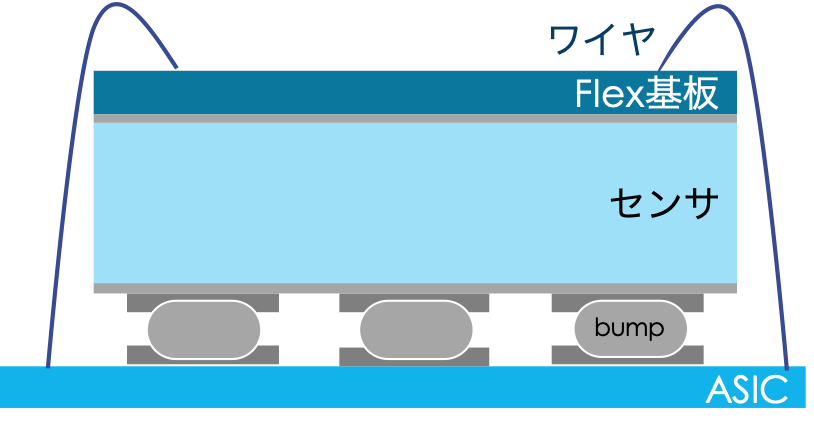
\includegraphics[width=8cm]{./figure/module.png}
  \caption{ピクセル検出器の概念図}
  \label{fig:module}
\end{figure}

\section{シリコンピクセルセンサ}
\label{sec:sensor}
この節では,ピクセル検出器を構成する要素の1つであるシリコンピクセルセンサについて説明する.

\subsection{シリコンピクセルセンサの原理}
シリコンセンサの動作原理は半導体に従う.この節では,半導体の基本原理と性質について述べる.\par
物質は導体,絶縁体,半導体の3種に分類することができる.これは,電気抵抗値によって決まっており,半導体は導体と絶縁体の中間の値をもつ.一般に室温で,$10^{-2}$から$10^9 \mathrm{\Omega cm}$の範囲に分類される.典型的な半導体物質にはシリコン,ゲルマニウム,ガリウムヒ素などがあげられる.

\subsubsection*{ドナーとアクセプタ}
半導体に不純物をドープすると,不純物準位が生じる.図\ref{fig:Donner}は$\ce{Si}$原子が5個の価電子を有する$\ce{As}$に痴漢された状況を模式的に示した図である.$\ce{As}$原子は隣接する4個の$\ce{Si}$原子と共有結合を形成し,残った電子は$\ce{As}$原子と弱く結合することで,適度な温度でイオン化されて伝導電子になる.この時の$\ce{As}$原子をドナーと呼ぶ.$\ce{Si}$は負電荷を持ったキャリアの負荷によりn型の半導体となる.同様に図\ref{fig:Acceptor}は3個の価電子をもつ$\ce{B}$が$\ce{Si}$に置換した場合を示す.4個の共有結合が$\ce{B}$の周囲にできるため,電子が1個取り込まれ,価電子帯に正に帯電した正孔が生じる.これがp型の半導体であり,$\ce{B}$はアクセプタと呼ばれる.

\begin{figure}[h]
  \centering
  \begin{minipage}[b]{0.45\linewidth}
    \centering
    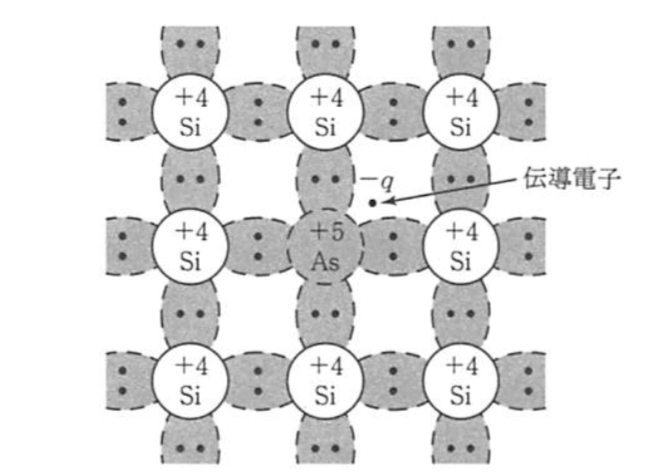
\includegraphics[width=8cm]{./figure/donner.png}
    \subcaption{ドナーをドープしたn型$\ce{Si}$}
    \label{fig:Donner}
  \end{minipage}
  \begin{minipage}[b]{0.45\linewidth}
    \centering
    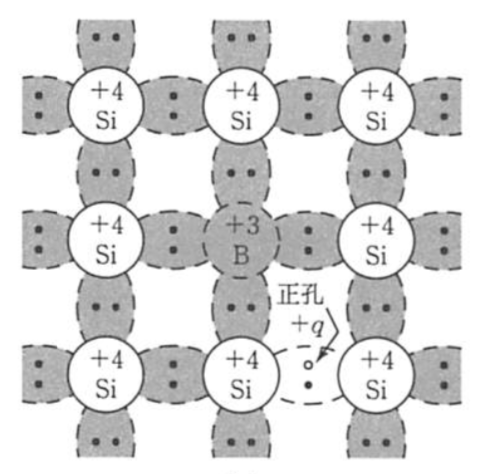
\includegraphics[width=5.8cm]{./figure/accepta.png}
    \subcaption{アクセプタをドープしたp型$\ce{Si}$}
    \label{fig:Acceptor}
  \end{minipage}
  \caption{ドープした半導体}
\end{figure}


\subsubsection*{pn接合と空乏化}
p型とn型の半導体が結合されると,接合部における大きなキャリア密度の勾配によってキャリアの拡散が起こる.p側からn側に向けて正孔が,n側からp側に向けて電子が拡散する.正孔がp側から拡散すると,結晶格子に固定されている負のアクセプタイオンが中和されずに接合近傍に残る.同様に,電子がn側から移動すると正のドナーイオンが接合近傍に残る.その結果,接合のp側には負の空間電荷が,n側には正の空間電荷が形成される.この空間電荷によって,電解が発生し,その向きは図\ref{fig:pn}のように正電荷側から負電荷側に向いている.\par

\begin{figure}[h]
  \centering
  \begin{minipage}[b]{0.45\linewidth}
    \centering
    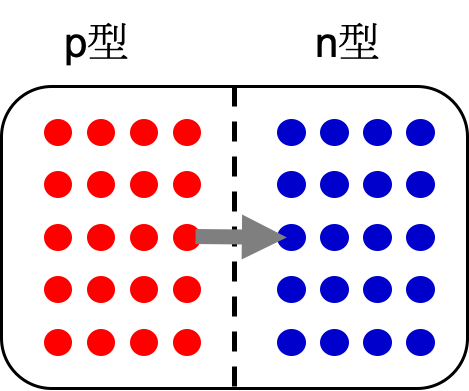
\includegraphics[width=4cm]{./figure/semiku1.png}
    \subcaption{過剰な電子と正孔が集まる}
  \end{minipage}
  \begin{minipage}[b]{0.45\linewidth}
    \centering
    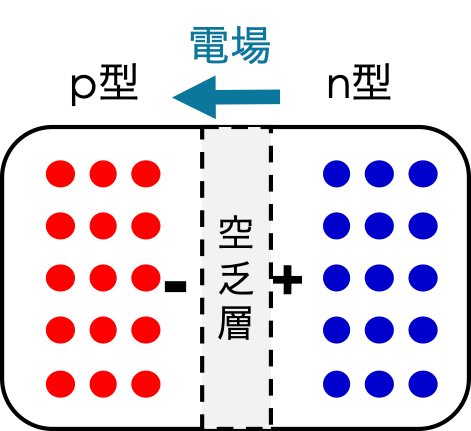
\includegraphics[width=4cm]{./figure/semiku2.png}
    \subcaption{空乏層が形成される}
  \end{minipage}
  \caption{pn接合半導体の空乏層概念図}
  \label{fig:pn}
\end{figure}


中世領域から接合部に近づくと,狭い遷移領域を経た上で,キャリアが存在しない領域が存在する.この領域を空乏層と呼ぶ.この空乏層の両端に生じる電位差は内臓電位$V_{bi}$と呼ばれ,アクセプタ濃度$N_A$,ドナー濃度$N_B$,不純物を含まない真性キャリア濃度$n_i$を用いて,式\ref{eq:bias}のように表される.\par
\begin{eqnarray}
  \label{eq:bias}
  V_{bi} = \frac{kT}{q} \ln \left( \frac{N_A N_D}{n_i^2} \right) 
\end{eqnarray}

空乏層幅は,静電ポテンシャルを示した一次ポアソン方程式\ref{eq:poisson}を解くことで,式\ref{eq:width}のような内部電位の関数にて表される.
\begin{eqnarray}
  \label{eq:poisson}
  \frac{d^2\Psi}{dx^2} \equiv -\frac{dE}{dx} = - \frac{q}{\epsilon_s}(N_D - N_A + p - n) \\
  \label{eq:width}
  W = \sqrt{ \frac{2\epsilon_s}{q} \left( \frac{N_A+N_D}{N_A N_D} \right) V_{bi}}
\end{eqnarray}

シリコンセンサはドープ量の少ない半導体にドープ量の多い半導体をインプラントしている($N_A \gg N_D$)ので,p側の空乏層幅はn側と比較して十分小さくなる.よって,式\ref{eq:width2}のように簡単に表すことができる.
\begin{eqnarray}
  \label{eq:width2}
  W \sim \sqrt{ \frac{2\epsilon_s V_{bi}}{q N_D} }
\end{eqnarray}

\subsubsection*{荷電粒子の検出}
荷電粒子が物質中の電子との衝突によって失うエネルギーは,Bethe-Blochの式\ref{eq:bb}で表される.\par
\begin{eqnarray}
  \label{eq:bb}
  - \frac{dE}{dx} = K z^2 \rho \frac{Z}{A} \frac{1}{\beta^2} \left[ \ln \left( \frac{2m_e c^2 \beta^2 \gamma^2 W}{I^2} \right) - \beta^2 - \frac{\delta(\gamma)}{2} \right]
\end{eqnarray}

入射した荷電粒子は物質中を通過する際に,物質の電子と相互作用することで,イオン化・励起し,電荷を生成する.この電荷をセンサが収集することで,通過した荷電粒子のエネルギーを知ることができる仕組みになっている.式\ref{eq:bb}より,$\beta \gamma \sim 3$付近で$-dE/dx$は最小となる.このような粒子をMinimum Ionization Particle(MIP)と呼ぶ.ここで,1MIPが150 $\mu m$厚のシリコンセンサを通過した場合を考える.MIPはシリコン中で多数の電子と相互作用し,その時に失うエネルギーの分布は式\ref{eq:landau}のようなランダウ分布になる.
\begin{eqnarray}
  \label{eq:landau}
  f(\lambda) = \frac{1}{\pi} \int ^{\infty} _0 \exp[-t (\ln t+\lambda) ] \sin(\pi t) dt
\end{eqnarray}

今回の場合の最頻値は,平均値の約0.7倍,シリコン中でのMIPのエネルギー損失の平均は,1.664 $\mathrm{MeV cm^2/g}$,シリコンの密度は2.329 $\mathrm{g/cm^3}$である.したがって,1MIPが損失するエネルギーは式\ref{eq:Emip}のように表せる.

\begin{eqnarray}
  E &=& 1.664 \times 3 \times 10^{-2} \times 2.329 \times 0.7 \nonumber \\
  \label{eq:Emip}
  &=& 8.14 \times 10^4 \mathrm{eV}
\end{eqnarray}

また,電子-正孔対生成に必要なエネルギーは3.62$\mathrm{eV}$であるから,生成され電子-正孔対の数は式\ref{eq:thr}のようになる.
\begin{equation}
  \label{eq:thr}
  E / 3.62 = 22500
\end{equation}


\subsection{バイアス構造}
シリコンピクセルセンサには,製造時に良品不良品を選別するための高電圧用のバイアス構造が備わっている.\par
バンプボンディングの前にセンサのみの試験を行い,動作不良センサを取り除く品質評価の工程がある.このピクセルセンサ評価方法として,IV測定がある.IV測定には全てのピクセルがGNDに落とされている必要があり,また,各ピクセルは分離されている必要がある.そのための構造がバイアスレールとPolySi抵抗である.ピクセル間にバイアスレールを起き,そこから各PolySi抵抗を引くことで,各ピクセルはGNDと同電位とすることができ,各ピクセルは抵抗によって分離される.\par

\subsection{今回使用したシリコンピクセルセンサ構造}
本論文で扱うピクセルセンサの表面構造について述べる.図\ref{fig:sensor}は,上から見たセンサの様子である.ピクセルセンサは2次元的に電極が配列されており,センサのみのテストのためにバイアスレールが敷かれている.本論文で用いたピクセルセンサは図\ref{fig:sensor}で示すように,row番号0-96はバイアスレールが存在せず,col番号96-192はバイアスレールが存在する構造になっている.

\begin{figure}[h]
  \centering
  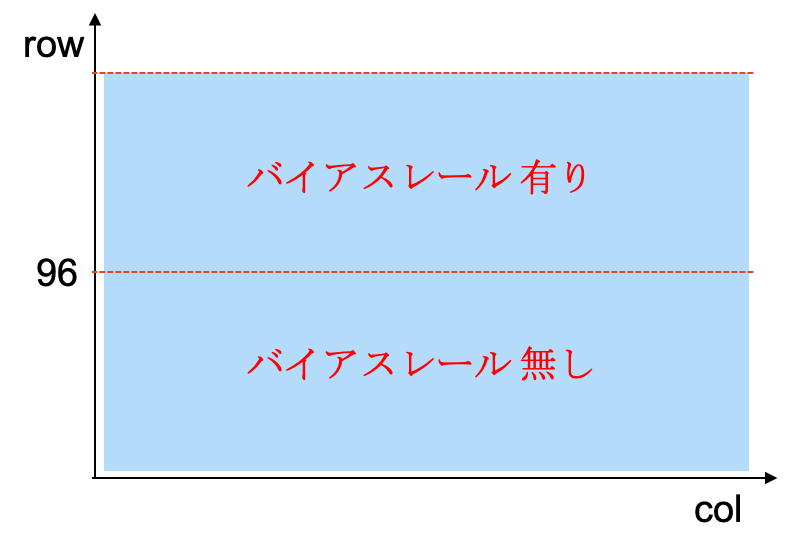
\includegraphics[width=7cm]{./figure/sensor.png}
  \caption{センサの構造.バイアスレールの有無}
  \label{fig:sensor}
\end{figure}


\section{HL-LHC ATLAS実験用新型ASIC・RD53A}
\label{sec:rd53a}
この節では,モジュールを構成する要素の1つであるASICについて述べる.ピクセル検出器からの信号は,検出器に直接接続された電気回路で最初に処理される.この電気回路をフロントエンドエレクトロニクスと呼ぶ.この回路は,全て専用の信号読み出し用ASIC内に実装されている.そのため,フロントエンドASICと呼ぶこともあるが,以降ではASICと呼ぶことにする.この回路を用いて検出器からの微弱な電気信号を受け取り,計測用のシステムに最適化した応答をするように信号をアンプ回路や波形整形回路などで調整する.さらに,コンピュータでの解析処理や,データの保存のためにアナログ信号をデジタル信号に変換する.\par
本論文で用いたASIC・RD53AはHL-LHC ATLAS実験用に開発されたプロトタイプ版の新型ASICであり,前章で述べたような,高い放射線耐性と,高い位置分解能を達成する.以下に現行のATLAS検出器で用いられているASIC・FEI4とFEI3,プロトタイプ版新型ASIC・RD53Aの比較を示す.

\begin{table}[h]
  \centering
  \caption{現行のASIC2種と新型プロトタイプ版ASICの比較}
  \begin{tabular} {|l|cc|c|} \hline
    ASIC名 & FEI3 & FEI4 & RD53A \\ \hline \hline
    ピクセルサイズ & 50 $\times$ 400 $\mathrm{\mu m^2}$ & 50 $\times$ 250 $\mathrm{\mu m^2}$ & 50 $\times$ 50 $\mathrm{\mu m^2}$ \\
    ピクセルのチャンネル数 & 18 $\times$ 160 & 80 $\times$ 336 & 50 $\times$ 50 $\mathrm{\mu m^2}$ \\ 
    チップサイズ & 7.6 $\times$ 10.8 $\mathrm{mm^2}$ & 20.2 $\times$ 19.0 $\mathrm{mm^2}$ & 20 $\times$ 11.8 $\mathrm{mm^2}$\\ \hline
  \end{tabular}
  \label{tab:ASIC}
\end{table}


\subsection{レジスタ}
ASICには,アナログ回路とデジタル回路の振る舞いを調節するために,回路の動作を制御する設定値を保持するレジスタが存在する.RD53Aのレジスタは2種類存在し,全てのピクセルに共通の設定を保存するグローバルレジスタ(GR)と各ピクセルの設定値を保持するピクセルレジスタ(PR)がある.
\begin{itemize}
\item グローバルレジスタ\\
  RD53Aには137個のGRがあり,ピクセルに共通が閾値(threshold),回路のオンオフなどを設定することができる.
\item ピクセルレジスタ\\
  Synchronous Frontendには3 $\mathrm{bit}$,その他の2つのフロントエンドには8 $\mathrm{bit}$のレジスタがある.ピクセルのデジタル回路のオンオフや閾値(threshold)を設定することができる.
\end{itemize}


\subsection{RD53Aフロントエンドデザイン}
RD53Aはプロトタイプ版のため,Synchronous Frontend, Linear Frontend, Differential Frontendと,3つの異なるフロントエンドデザインが存在する.

\begin{figure}[h]
\centering
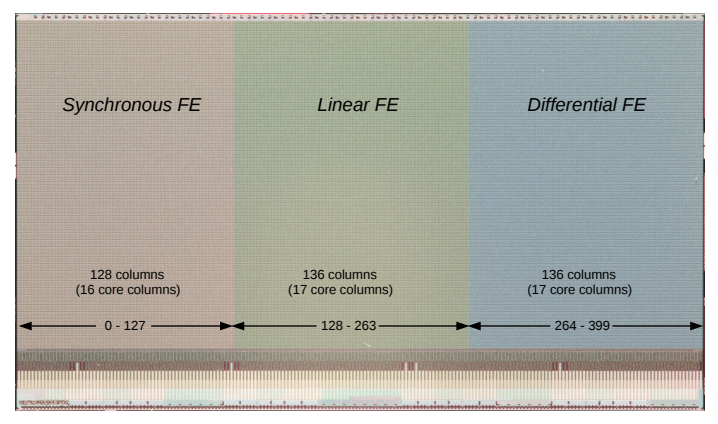
\includegraphics[width=8cm]{./figure/RD53A_FE.png}
\caption{RD53Aのフロントエンドデザイン}
\label{fig:RD53AFE}
\end{figure}

今回は実機で利用されることが予定されているDifferential Frontend(以下:Diff FE)のみを用いて研究を行なったため,それについて詳しく説明する.

\subsubsection*{Diff FEの仕組み}
3つのフロントエンドで大きく異なるのは,アナログ回路部分の構造である.Diff FEのアナログ回路構造を以下に示す.\par

\begin{figure}[h]
\centering
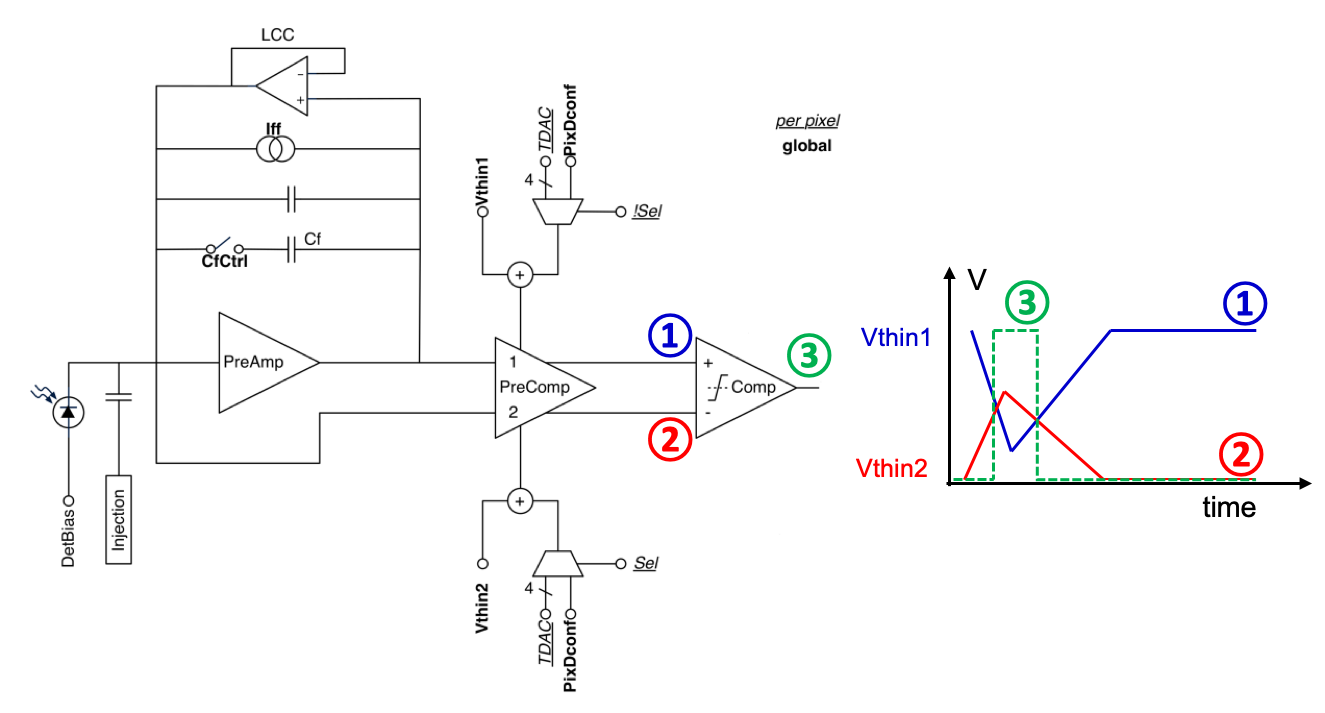
\includegraphics[width=12cm]{./figure/RD53A_DiffFE.png}
\caption{Diff FEのアナログ回路構造}
\label{fig:DiffFE}
\end{figure}

図\ref{fig:DiffFE}に示したように,Diff FEでは,RD53AのGR値である''DiffVthin1''と''DiffVthin2''で閾値を設定可能である.これらのGR値は,入力された信号(図\ref{fig:DiffFE}の赤い信号)と,それに対して反転増幅を行なった後の信号(図\ref{fig:DiffFE}の青い信号)それぞれに作用するオフセット電圧である.Diff FEはこれらの信号の差動によって,出力信号を定義しているため,オフセットを変化させることで,閾値を調整することができる.また,GR値である''DiffLccEn''で図中のCfCtrlのスイッチのオンオフを,''DiffLcc''でLCC回路に印加する電圧を設定することができる.

\subsection{RD53Aのデータ収集の仕組み}

\begin{figure}[h]
  \centering
  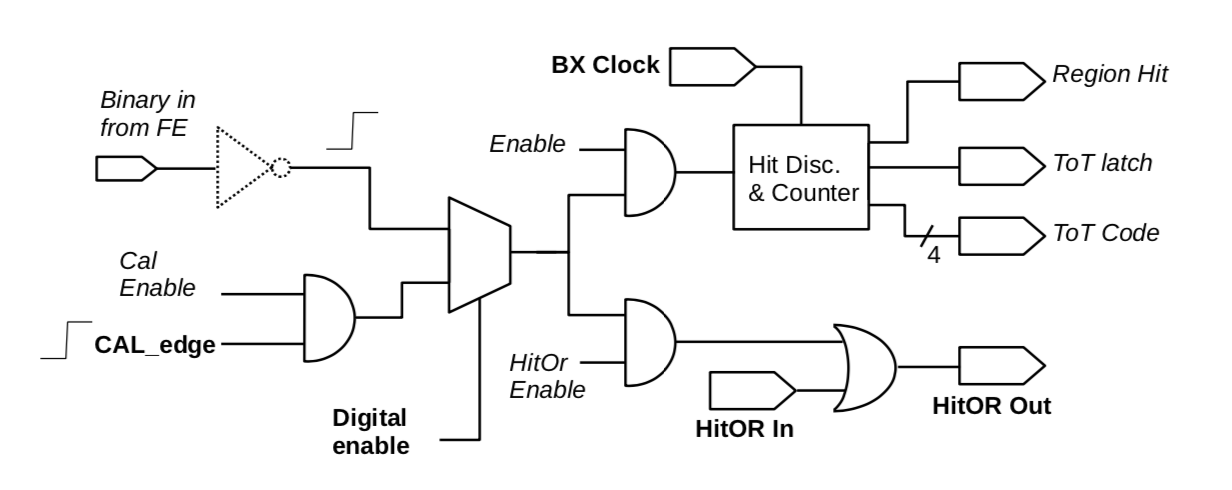
\includegraphics[width=13cm]{./figure/RD53Aproc.png}
  \caption{RD53Aのデータ収集の仕組み.全ピクセルに共通する信号が太字,ピクセルごとに記録されている信号が斜体文字になっている.}
  \label{fig:RD53Aproc}
\end{figure}

図\ref{fig:RD53Aproc}にRD53Aのデータ収集の仕組みを示す.まず,Hitとされる信号(センサからの信号)はBinary in from FEから,擬似パルスによる信号はCALedgeから入射する.各ピクセルごとに設定されている''Enable''がオンの場合,そのピクセルのデータは図中のHit Disc. \& Counterに入る.ここでは,Hitを検出したピクセルの位置(Region Hit)と,40$\mathrm{MHz}$のBX Clockに合わせて数え上げられるToT値とLatency値が記録されていく.

\subsubsection*{Time over Threshold(ToT)}
ToTとは,図\ref{fig:tot}で示すように,信号(Signal)が閾値(Threshold)を超えている間の時間を指す.

\subsubsection*{Latency}
Latencyとは,図\ref{fig:tot}で示すように,トリガが入力されてからどれだけ時間を遡ってデータ読み出しを行うかを指定する値をさす.

\begin{figure}[h]
  \centering
  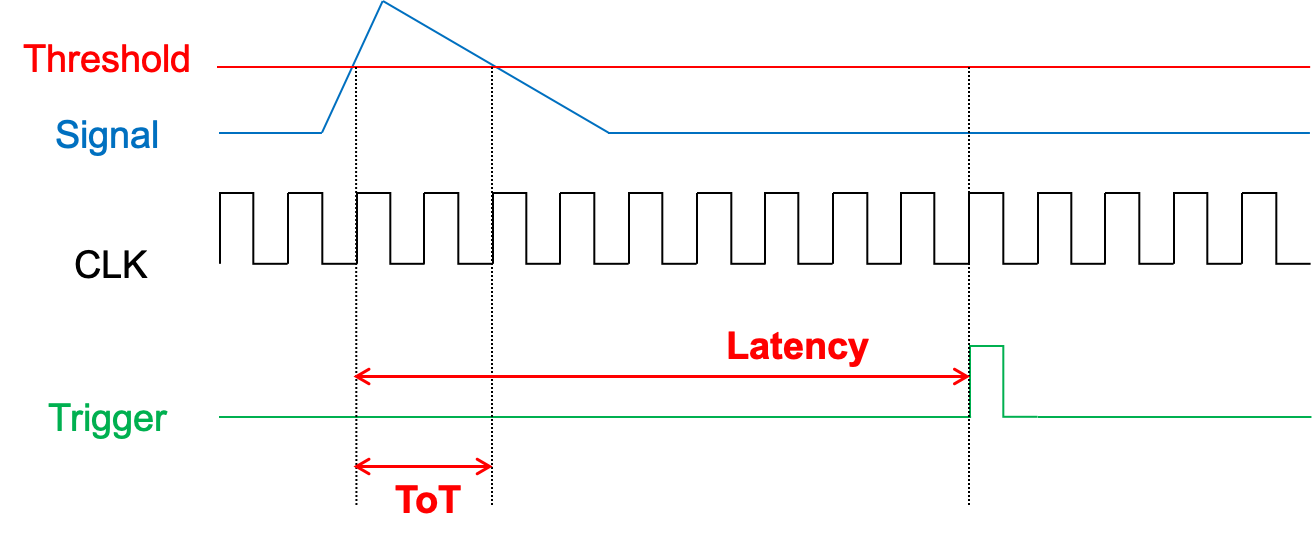
\includegraphics[width=13cm]{./figure/tot.png}
  \caption{信号が入力された時のToTとLatency}
  \label{fig:tot}
\end{figure}



\subsection{HitOR信号}
RD53Aには,現行のFEI4に実装されているセルフトリガ機能がない代わりに,HitORというセンサに荷電粒子が入射したタイミングで,出力される信号が存在する.HitOR信号出力する仕組みについて説明する.図\ref{fig:RD53Aproc}において,各ピクセルで設定されているレジスタ''HitOr Enable''がオンの場合,Hit信号または擬似パルス信号が入射すると,Hit Disc. \& Counterに入るのと同時に図中右下のHitOR Outから信号が出力される.これがHitOR信号である.\par

\begin{figure}[h]
  \centering
  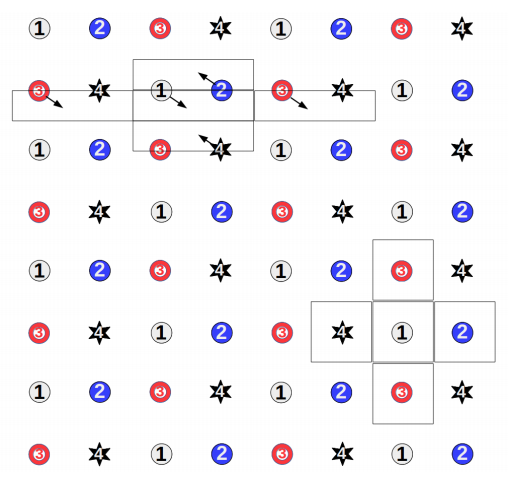
\includegraphics[width=8cm]{./figure/HitOR.png}
  \caption{HitOR信号のネットワーク図}
  \label{fig:HitOR}
\end{figure}

HitOR信号は4つのネットワークによって出力される.図\ref{fig:HitOR}はRD53Aの一部である$8 \times 8 \mathrm{pixel}$を示している.HitOR信号は,図\ref{HitOR}の各ピクセルに割り当てられている番号1-4ごとにまとめて読み出される.これを番号ごとにネットワークと呼ぶ.このネットワークは任意のネットワークに含まれるピクセルの上下に1つのネットワーク,左右に異なる2つのネットワークが存在するように配置されている.例えば,1番のネットワークのあるピクセルには,3番のネットワークが上下に存在し,左右には2番と4番のネットワークが存在するようになっている.このように配置されたネットワークごとに,HitORは読み出される仕組みになっている.

\section{モジュール量産に向けた品質性能試験}
\label{sec:moduletest}
量産されたモジュールは品質性能基準を達成するために,試験にかけられる.その試験項目の1つとして,本論文に関わる,粒子線に対する応答評価試験が存在する.

\subsection{粒子線に対する応答評価試験の意義}
HL-LHC ATLAS実験に向けたピクセル検出器量産に際して,全ての検出器モジュールに対して,品質管理のための試験を行う.この試験項目の1つとして,粒子線に対する応答評価試験が設けられている.前章でも述べたように,ピクセル検出器の各チャンネルとASICはバンプボンディングという手法で接続されている.このバンプボンディングに異常がないかどうかを確認するための試験が,ソーススキャンである.\par

\subsection{応答評価試験の手法}
応答評価試験には,主に2種類の手法がある.1つは,センサに荷電粒子が入射した時の信号を取得したタイミングでデータ取得を行う,セルフトリガと呼ばれる手法.もう1つは,センサの上にシンチレータ,その上に粒子線源を設置し,シンチレータに粒子線が入射した時の信号を取得したタイミングでデータ取得を行う手法である.今回はこれら2種類の手法を用いて応答評価試験を行い,どのような試験結果の振る舞いがなされるかの検証を行なった.\par
YARRソフトウェアには,外部トリガスキャンという機能が実装されているため,今回はこの外部トリガにHitOR信号を用いた手法をセルフトリガ,シンチレータに粒子線が入射した時の信号を用いた手法を外部トリガと呼ぶ.

\subsection{本研究の目的}
本研究では,シリコンピクセルセンサが接続されたHL-LHC ATLAS実験用新型ASIC搭載モジュールを用いて,2種類の手法で行なったの粒子線に対する応答評価試験結果について報告する.

\chapter{粒子線に対する応答評価試験のための読み出しシステムの動作確認}
本研究では,粒子線に対する応答評価試験のため,ファームウエアに外部トリガを処理する機能の追加を行なった.この章では,\ref{sec:setup}節で読み出し試験のセットアップ概要,\ref{sec:scans}節で機能を追加したファームウェアが正しく動作しているかの確認について述べる.

\section{読み出しセットアップ概要}
\label{sec:setup}
以下に読み出しシステムの概要を示す.主にRD53A搭載のSingle Chip Card(SCC)とFPGAボード,PCを用いて読み出しシステムを構成している.今回は読み出しASICとFPGAボードは,HPC-mDP変換ボードを用いてケーブルにて接続を行い,FPGA内部でASICからのデータ信号の処理を行なった.また,高速通信用インターフェースでPCとFPGAボードを接続し,データ転送を行なった.\par

\begin{figure}[h]
  \centering
  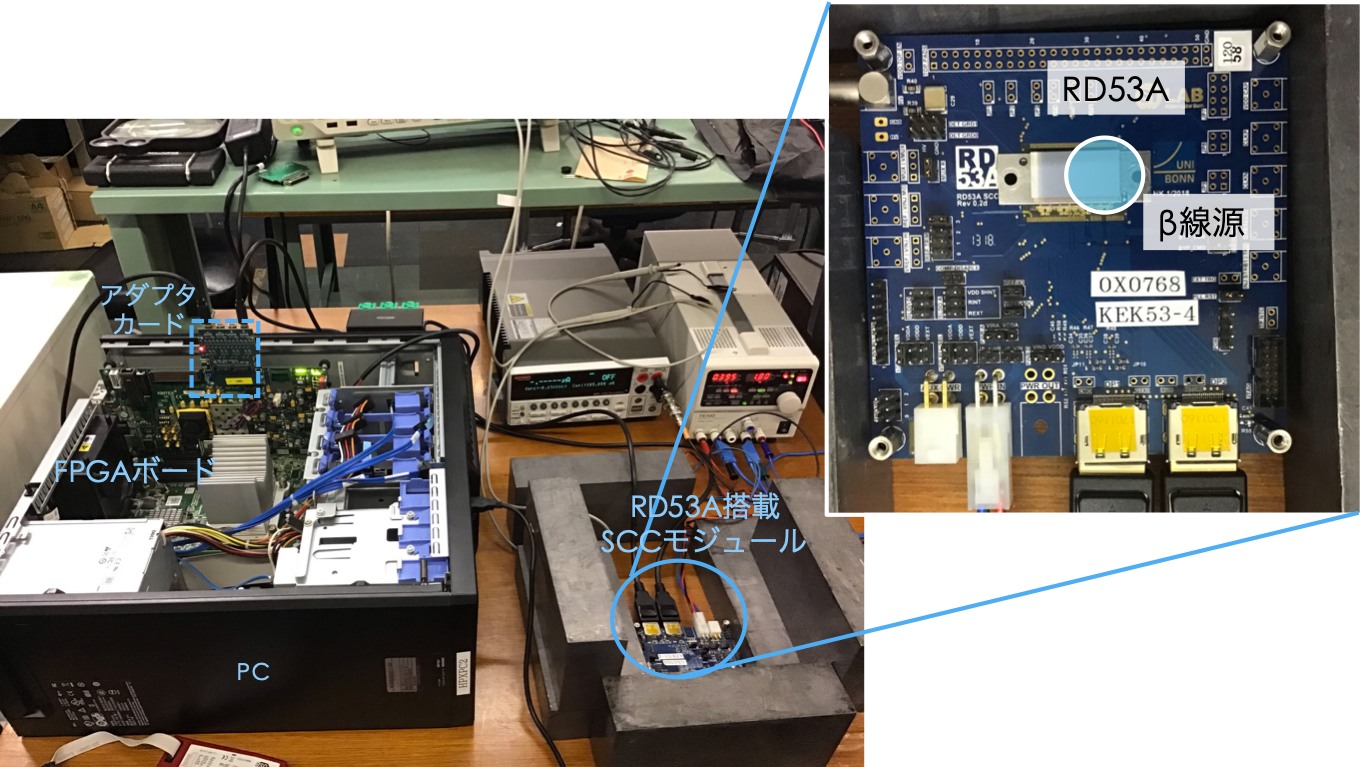
\includegraphics[width=15cm]{./figure/Setup.png}
  \caption{セットアップ}
  \label{fig:setup}
\end{figure}

\subsection*{PC}
PCからPCIeによって接続されたFPGAボードに制御コマンドを送る.また,FPGAボードからきたデータを整理する.DAQの基本的なソフトウェアとファームウェアはYARRのDAQシステムを用いた.YARRとは読み出しシステムの構築と性能向上を目指すオープンソースプロジェクトである.

\subsection*{FPGAボード}
Xilinx, Inc.のKintex-7 FPGA搭載KC705評価ボードを使用した.このFPGAボードは,研究室規模の実験で使うことを想定していることから,一般的に流通していて入手性がよいため,このFPGAボードを使用している.また,KC705はPCIe通信に対応し,PCとPCIe間では5.12 $\mathrm{Gbps}$の通信速度に対応している.今回はYARRのシステムに外部トリガを受信,処理を行う機能を追加し,RD53Aの出力するHitOR信号を用いて,外部トリガを受信できているかを確認した.

\subsection*{アダプタカード}
ASICはDP-mDPケーブルからmDP-HPCアダプタカードを通してFPGAボードに接続される.

\subsection*{RD53A搭載Single Chip Cardモジュール}
ASICを1チップ搭載した試験用モジュールがSingle Chip Cardモジュールである.今回試験したのはアップグレード用のプロトタイプ版ASICであるRD53A搭載のモジュールである.センサ付きのRD53Aが搭載されたモジュールの写真を以下に示す.
RD53Aは細い金属ワイヤにより基板上の回路パターンと電気的に接続されている.基板にRD53Aが外部と通信するためのDPコネクタ(図中:DP1),電源供給のためのmolexコネクタ(図中:PWR IN),センサに電圧を印加するためのLEMOコネクタ(図中:HV),センサが検出した信号を外部に出力するためのDPコネクタ(DP2)が実装されている.
\begin{figure}[h]
  \centering
  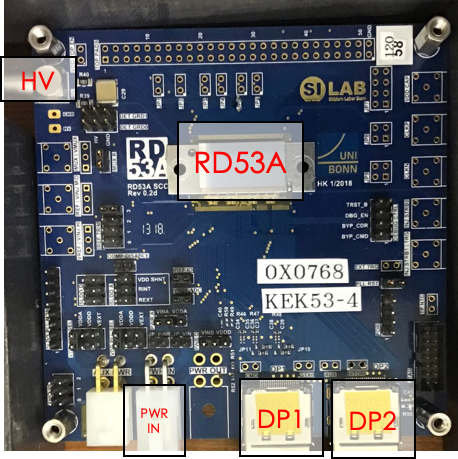
\includegraphics[width=7cm]{./figure/rd53a.png}
  \caption{センサ付きRD53A搭載Single Chip Cardモジュール}
  \label{fig:scurve}
\end{figure}

今回電源とセンサに印加した電圧は\ref{tab:voltage}に示す.

\begin{table}[h]
  \centering
  \caption{今回RD53Aとセンサに供給した電圧}
  \begin{tabular} {|l|cc|c|} \hline
     & RD53A & RD53A & ピクセル \\ 
     & アナログ回路 & デジタル回路 & センサ \\ \hline
    印加電圧[$\mathrm{V}$] & 1.80 & 1.80 & -50 \\ \hline
  \end{tabular}
  \label{tab:voltage}
\end{table}


\subsection*{$\beta$線源}
今回は粒子線として$\beta$線源であるストロンチウム90を使用した.ストロンチウム90は中性子過剰であるため,$\beta$崩壊によってイットリウム90を生成し,その後さらなる$\beta$崩壊によってジルコニウム90となる.半減期は28.79年であるが,2段階の$\beta$崩壊が起こるため,$\beta$線のエネルギーは高いものになっている.式\ref{eq:beta}にベータ崩壊の機構を,式\ref{eq:sr90}にストロンチウムの崩壊過程を示す.\par
\begin{equation}
  \label{eq:beta}
  n \rightarrow p^{+} + e^{-} + \overline{\nu_e}
\end{equation}
\begin{equation}
  \label{eq:sr90}
  \ce{^{90}Sr} \rightarrow \ce{^{90}Y} \rightarrow \ce{^{90}Zr}
\end{equation}


$\beta$線の今回用いた$\beta$線源は2017/02/13時点で$ 5.00 \times 10^3 \mathrm{Bq}$のものであった.すなわち現在の放射能は以下のように求められる.

\begin{equation}
\label{eq:radiation}
  A = -\lambda N_1 = A_0 \exp \left( - \frac{\ln 2}{T} t \right)
\end{equation}

ここで,
\begin{table}[h]
  \centering
  \begin{tabular}{cc} \hline
    $A_0$ & 2017/02/13時点での放射能($ 5.00 \times 10^3 \mathrm{Bq}$)\\
    $T$ & \ce{^{90}Sr}の半減期(28.79 $\mathrm{year}$)\\
    $t$ & 2017/02/13から現在までの時間(25/12 $\mathrm{year}$)\\ \hline
  \end{tabular}
\end{table}


式\ref{eq:radiation}より,現在の放射能$A$は,$4.76 \times 10^3 \mathrm{Bq}$と求まる.
  

%\begin{table}[h]
%  \centering
%  \caption{今回使用した$\beta$線源の放射能}
%  \begin{tabular}{|l|c|} \hline
%    基準日 & 2017/02/13 \\
%    放射能 & 5.00 $\times 10^3 \mathrm{Bq}$ \\ \hline
%  \end{tabular}
%  \label{tab:beta}
%\end{table}



\section{伝達確認}
\label{sec:scans}
ソーススキャンを行うために,既存のKC705用YARRファームウェアに外部トリガを処理する機能を追加した.本節では,機能を追加したファームが外部トリガの受信確認について述べる.

\subsection{コマンド信号とデータ信号の確認}
オシロスコープでコマンド信号とデータ信号をRD53A SCC上でプローブし,波形を確認した.

\begin{figure}[h]
  \centering
  \begin{minipage}[b]{0.45\linewidth}
    \centering
    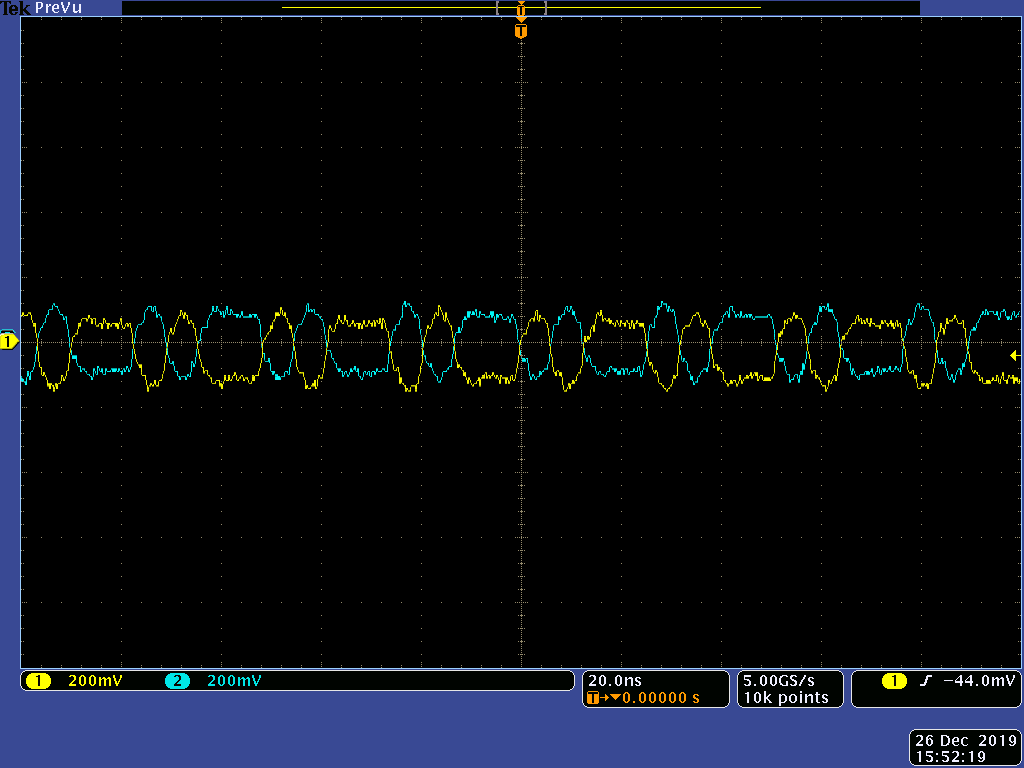
\includegraphics[width=6cm]{./figure/CMDLine.png}
    \subcaption{コマンド信号}
    \label{fig:cmd}
  \end{minipage}
  \begin{minipage}[b]{0.45\linewidth}
    \centering
    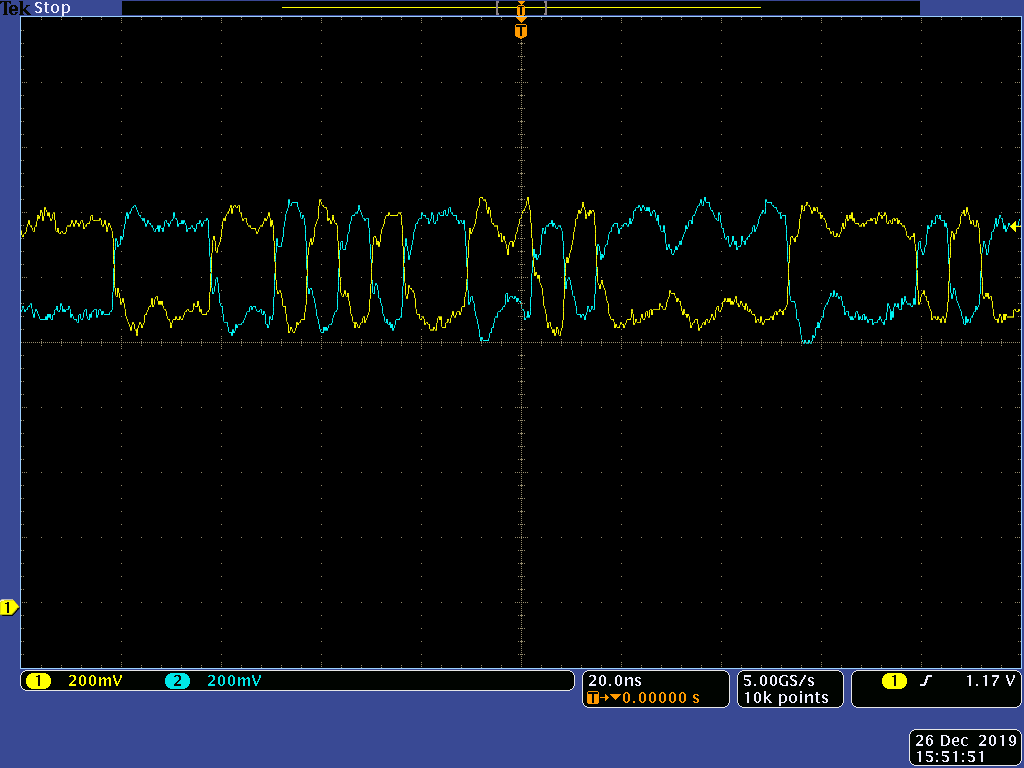
\includegraphics[width=6cm]{./figure/DataLine.png}
    \subcaption{データ線のアイドル信号}
    \label{fig:gtx}
  \end{minipage}
  \caption{コマンド信号とデータ信号のオシロスコープの波形}
\end{figure}

\subsection{デジタルスキャン}
全ピクセルのデジタル回路に複数回擬似パルスを注入して,注入した回数のうち何回応答が返ってくるのかを確認する.この作業をデジタルスキャンと呼ぶ.全ピクセルごとの回路の応答を確認し,データの転送線,FPGA内部の処理,PCへの通信の各経路でデータの損失がないことを確認するのに有効である.図\ref{fig:digital}に100回擬似パルスを注入した時の応答数の分布を示す.
\begin{figure}[h]
  \centering
  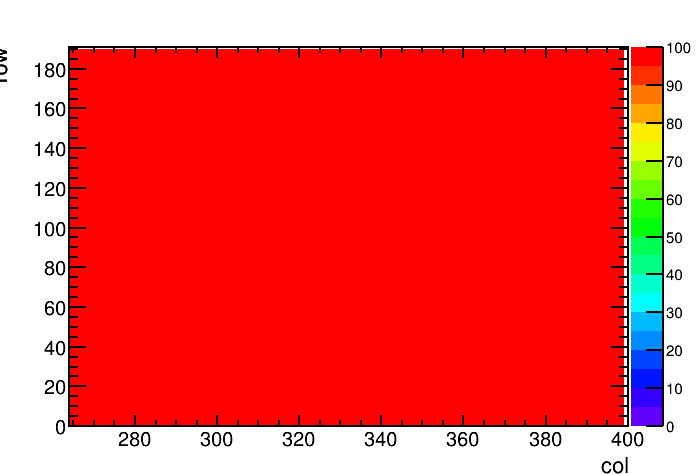
\includegraphics[width=7cm]{./figure/DigitalScan.png}
  \caption{デジタルスキャン}
  \label{fig:digital}
\end{figure}


\subsection{アナログスキャン}
アナログ回路に複数回擬似パルスを注入して,注入した回路のうち何回応答が返ってくるのかを確認した.この作業をアナログスキャンと呼ぶ.今回はDiff FEのみを使用するので,その他のフロントエンドは,グローバルレジスタの''EnCoreColSync1/2'',''EnCoreColEnLin1/2''を全て0にすることで非使用に設定した.この時,図\ref{fig:analog1}のように応答のない領域が存在した.これは,バイアスレールによりASICのプリアンプのVirtual GNDによる電位差でセンサのポリシリコン抵抗を介して電流が流れている影響だと考えられられており,Diff FEアナログ回路のLCC回路をオンにすることで改善することが知られている.本論文では,グローバルレジスタ値の''DiffLccEn''を0から1に変更し,''DiffLcc''を255にすることでLCC回路をオンにし,電圧をかけた.LCC回路をオンにした場合のアナログスキャンの様子を図\ref{fig:analog2}に示す.オフの場合と比較すると,応答のない領域が改善されているのがわかる.

\begin{figure}[h]
  \centering
  \begin{minipage}[b]{0.4\linewidth}
    \centering
    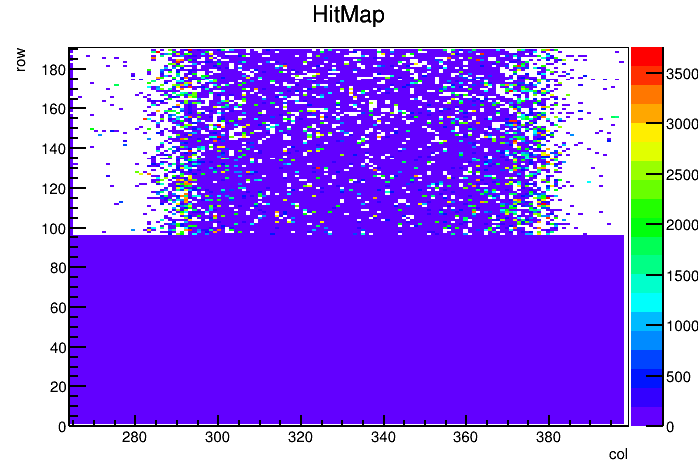
\includegraphics[width=6cm]{./figure/AnalogScan1.png}
    \subcaption{LCC回路をオフ}
    \label{fig:analog1}
  \end{minipage}
  \begin{minipage}[b]{0.4\linewidth}
    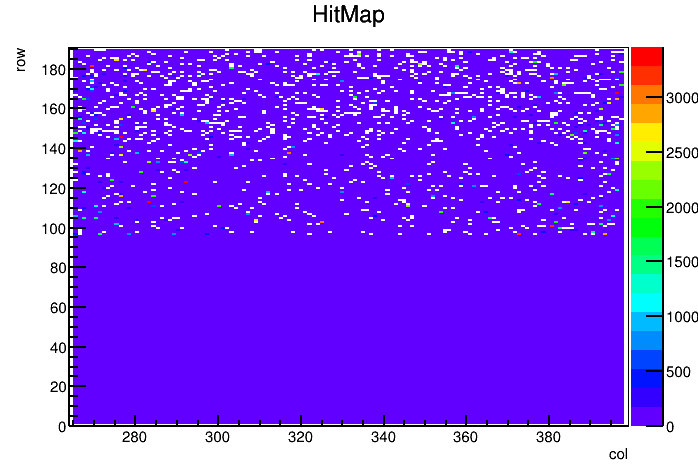
\includegraphics[width=6cm]{./figure/AnalogScan3.png}
    \subcaption{LCC回路をオン}
    \label{fig:analog2}
  \end{minipage}
  \caption{アナログスキャン}
\end{figure}


\subsection{閾値のチューニング}
\begin{figure}[h]
  \centering
  \begin{minipage}[b]{0.4\linewidth}
    \centering
    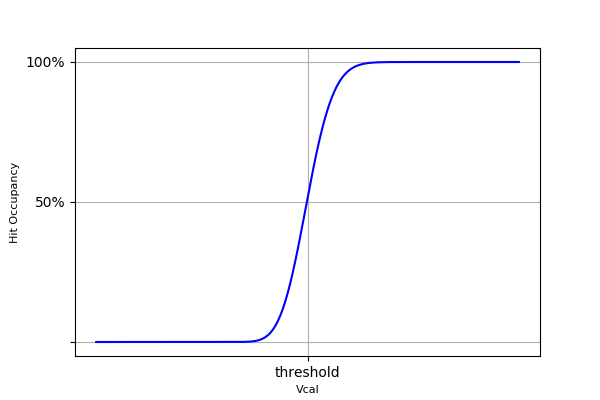
\includegraphics[width=7cm]{./figure/scurve.png}
    \subcaption{注入電荷$V_{cal}$と応答率の関係}
    \label{fig:scurve}
  \end{minipage}
  \begin{minipage}[b]{0.4\linewidth}
    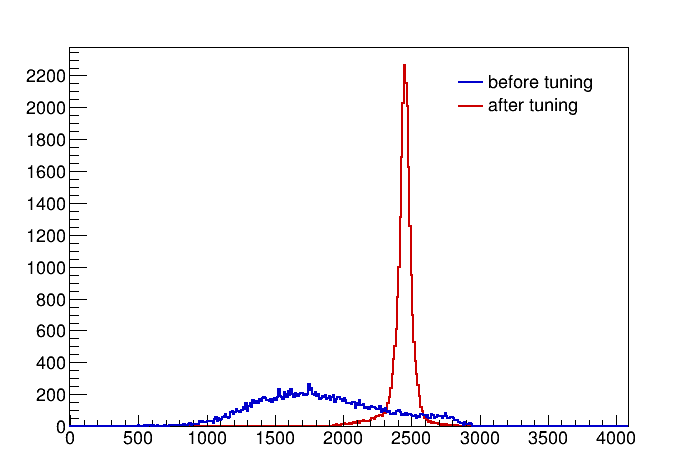
\includegraphics[width=7cm]{./figure/ThreDiff.png}
    \subcaption{チューニング前後閾値分布}
    \label{fig:ThrDistBefore}
  \end{minipage}
  \caption{閾値チューニング}
\end{figure}

閾値とはピクセルの応答率が50$\mathrm{\%}$となる電荷量で定義され,閾値が目標値になるように各ピクセルのDAC値を調節する作業を閾値のチューニングという.信号が閾値を超えたかあどうかでヒットと認識するかどうかの判定を行なっているが,信号には正規分布に従うノイズが載るため,信号がヒットとして認識される閾値には幅がある.そのため,注入電荷を変化させながら,各ピクセルに試験電荷を複数回入射したときの応答数の関係は,図\ref{fig:scurve}のような曲線になる.この曲線をSカーブと呼び,これを誤差関数でフィッティングすることで,応答率が50 $\mathrm{\%}$となる閾値を求める.
\begin{eqnarray}
  f(Q_{inj}) &=& \frac{1}{2} \left( 1 + \rm{erf} \left( \frac{Q_{inj} - Q_{thr}}{\sqrt{2} \sigma} \right) \right) \\
  \rm{erf}(x) &=& 1- \frac{2}{\sqrt{\pi}} \int^x _0 e^{-t^2} dt
  \label{eq:scurve}
\end{eqnarray}


閾値チューニング前後の各ピクセルの閾値のヒストグラムを図\ref{fig:ThrDistBefore}に示す.目標値は2400$\mathrm{e}$と設定した.2400$\mathrm{e}$という閾値は,センサの厚みとノイズ信号の大きさを考慮した値である.今回使用したセンサの厚みは,150 $\mathrm{\mu m}$であり,式\ref{eq:thr}の厚み300 $\mathrm{\mu m}$の場合のおよそ$1/2$であるため,全て空乏化した場合に発生する信号は10000 $\mathrm{e}$である.まず,この信号をASICが読み出す際に,4分割されてしまったとしても,検出してほしいために閾値は2400 $\mathrm{e}$以下であることが望ましい.また,ノイズ$\sigma$の大きさに対して6-7 $\sigma$離れている必要があるため,バイアスレール有りの場合,$\sigma = 200 \mathrm{e}$と知られているため,1200 $\mathrm{e}$以上にすることが望ましい.閾値のヒストグラムを見ると,1200 $\mathrm{e}$にチューニングした場合は,1200 $\mathrm{e}$以下まで多く分布してしまっているため,今回は分布が1200 $\mathrm{e}$以上に収まるような,2500 $\mathrm{e}$を目標値としてチューニングを行なった.

\subsection{ノイズスキャン}
任意の周波数でトリガを発行し,その全トリガ数に対するのアナログ回路から何回応答が返ってくるのかを確認する.この作業をノイズスキャンと呼ぶ.ピクセルセンサが粒子線以外の信号に対して反応していないことを確認するために有効である.\par
この作業によって,粒子線以外の信号に対して反応している部分は非使用に設定される.引き続きDiff FEのみを使用した.任意の周波数でトリガを送り,その時のアナログ回路からの応答に対して,閾値を超えるものを非使用に設定する.この作業をノイズスキャンと呼ぶ.今回は5000 $\mathrm{Hz}$で5分間ノイズスキャンを3回行なった.以下にノイズスキャンを行う前と行なった後のOccupancy MapとEnable Pixel Mapを示す.図\ref{fig:enablemap}より,非使用になっているピクセルが上半分に集中しているのが見て取れる.これは,センサ単体の試験で必要となるバイアスレールの影響であり,バイアスレールが存在すると,図\ref{fig:noisedist}のように,ノイズが増えることが知られている.

\begin{figure}[h]
  \centering
  \begin{minipage}[b]{0.45\linewidth}
    \centering
    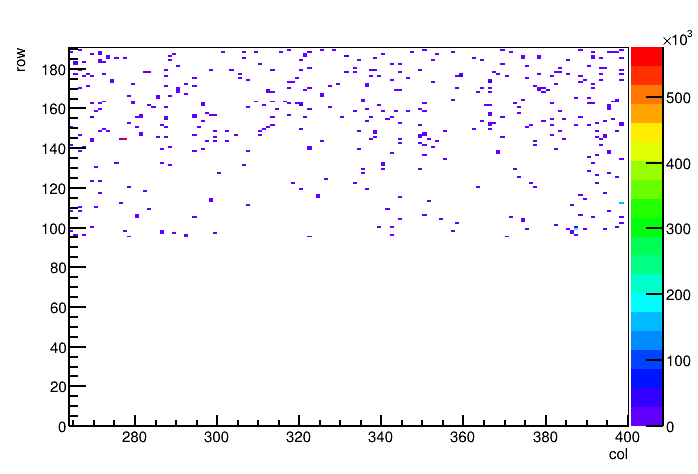
\includegraphics[width=7cm]{./figure/Noisebf.png}
    \subcaption{ノイズスキャン前}
    \label{fig:bfnoise}
  \end{minipage}
  \begin{minipage}[b]{0.45\linewidth}
    \centering
    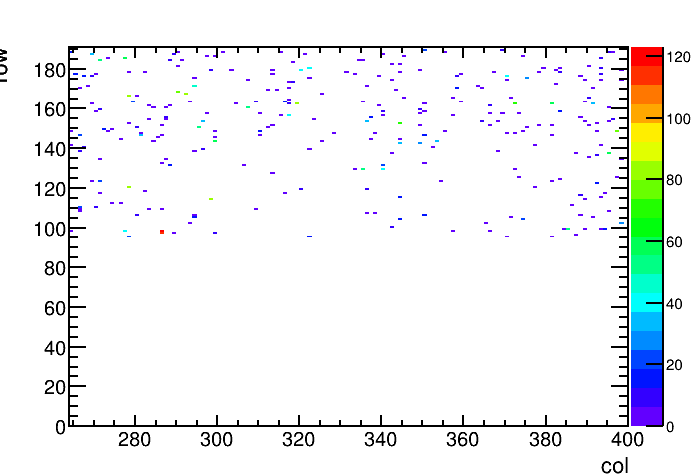
\includegraphics[width=7cm]{./figure/Noiseaf.png}
    \subcaption{ノイズスキャン後}
    \label{fig:afnoise}
  \end{minipage}
  \caption{Occupancy Map}
\end{figure}

\begin{figure}[h]
  \centering
  \begin{minipage}[b]{0.45\linewidth}
    \centering
    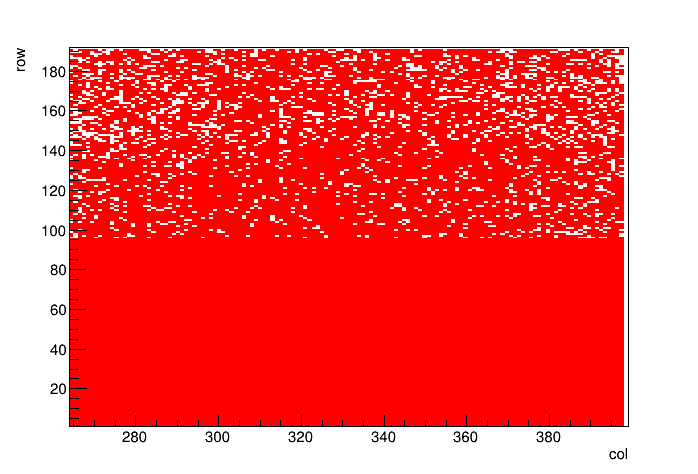
\includegraphics[width=7cm]{./figure/EnablePix.png}
    \subcaption{以降使用したピクセルの分布}
    \label{fig:enablemap}
  \end{minipage}
  \begin{minipage}[b]{0.45\linewidth}
    \centering
    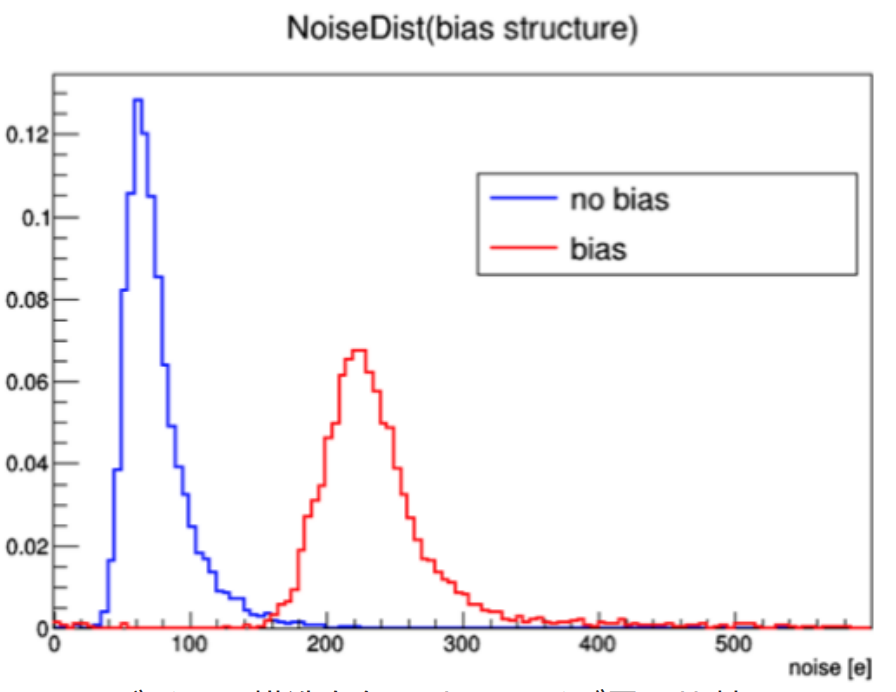
\includegraphics[width=6cm]{./figure/noisedist.png}
    \subcaption{バイアスレールの有無によるノイズ量比較}
    \label{fig:noisedist}
  \end{minipage}
  \caption{非使用なピクセルとバイアスレールによる影響}
\end{figure}


\subsection{HitOR信号の伝達確認}
モジュールの上に$\beta$線源を配置し,オシロスコープでHitOR信号をRD53A SCC上でプローブすることで,波形を確認した.また,FPGAまでHitOR信号が伝わっているかどうか,正常に処理され,そのタイミングでトリガが出力されているかどうかをVivadoのLogic Analyzerを用いて確認した.それが以下の図である.



このようにファームウェアに外部トリガを取得し,処理する機能を追加できていることを確認した.







\chapter{セルフトリガを用いた応答評価試験}
この章では,セルフトリガを用いた粒子線に対する応答評価試験について述べる.\ref{sec:latency}節で粒子線を用いた応答評価試験のために必要だったLatencyチューニング機能について述べ,そのあとに,\ref{sec:selfsetup}節で評価試験セットアップ,\ref{sec:selfhow}節で手順,\ref{sec:selfconc}節で取得データの結果を示し,\ref{sec:selfsum}節で考察を行なっている.

\section{Latencyチューニング機能の追加}
\label{sec:latency}
この節では,粒子線に対する応答評価のために必要だったLatencyチューニング機能について述べる.
\subsection{YARRにおけるトリガDAQとLatencyの意義}
YARRソフトウェアを用いたデータ取得におけるトリガDAQについて説明する図を図\ref{fig:YARRDAQ}に示す.\par
\begin{figure}[h]
  \centering
  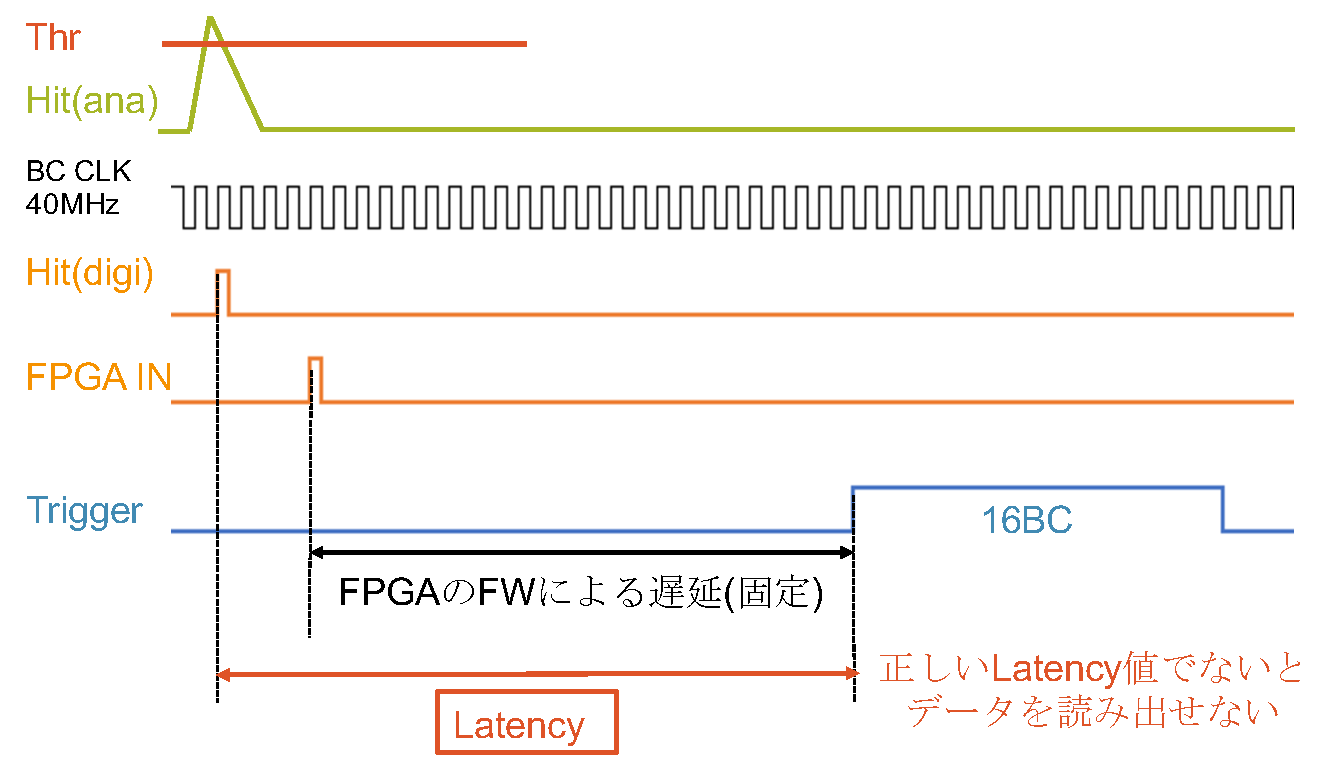
\includegraphics[width=13cm]{./figure/DAQ_signal.pdf}
  \caption{YARRトリガDAQ}
  \label{fig:YARRDAQ}
\end{figure}

Latencyとは,図のtrigger入力時にどれだけの時間遡ってメモリから情報を読み出すかを定める値である.このLatencyがずれていると,データを正しく読み出すことができない.YARRでは,指定されたLatency分遡ったClockの前7 $\mathrm{Clock}$,後8 $\mathrm{Clock}$,計16 $\mathrm{Clock}$分のデータを読み出す.16 $\mathrm{Clock}$の中で何 $\mathrm{Clock}$目のデータであるかを示す値として,L1IDというものが記録される.アナログスキャンにおけるL1IDの分布を以下に示す.\par
\begin{figure}[h]
  \centering
  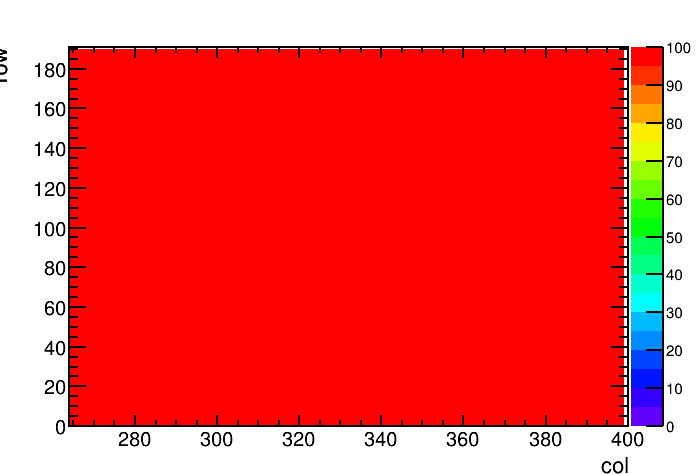
\includegraphics[width=8cm]{./figure/DigitalScan.png}
  \caption{YARRトリガDAQ}
  \label{fig:YARRDAQ}
\end{figure}


理想的にはL1IDが7のところにトリガの中心を合わせたい.そのために,YARRで指定できるLatencyに関する3種類のパラメータを以下に示す.
\subsubsection*{ソフトウェアで設定されている''delay''}
FPGAからトリガをどれだけ遅れて出力するかを決める値.本論文では,外部からトリガを受け取ってからどれくらい遅延させてFPGAからRD53Aにトリガを出力するかを決める値.

\subsubsection*{ファームウェアの設定値''delay''}
擬似パルスを送られてからどれくらい遅れてトリガを出力するかを決める値.前章で述べたデジタルスキャンやアナログスキャンの際に関係し,擬似パルスではなく外部からのトリガを使用してデータ取得するセルフトリガや外部トリガを用いたデータ取得の時には無関係.

\subsubsection*{グローバルレジスタ''LatencyConfig''}
RD53Aの全てのピクセルに共通する設定値であるグローバルレジスタの内の1つにLatencyConfigというLatencyに関する設定値が存在する.LatencyConfigがどのような値であるか説明する図を以下に示す.\par
ASICのあるピクセルが信号を検知すると,そのピクセルが40 $\mathrm{MHz}$のClockに合わせてカウントを始める.そして,FPGAから送られてくるトリガを受け取った時に,そのカウントが設定した''LatencyConfig''の値と等しいピクセルの情報を読み出すようになっている.''LatencyConfig''は,9bitの値であり,0-511まで変化させることが可能である.

\subsection{Latencyチューニング機能}
前節で述べたように,Latencyが合っていないと,データを正しく読み出すことができないので,Latencyを正しい値にすることが,データを正しく読み出す上で大変重要となる.そこで,今回はグローバルレジスタ''LatencyConfig''値を変化させることで,Latencyを合わせられるような機能をYARRに追加した.\par
今回,センサからの信号をASICがHitOR信号として出力したTriggerに対するLatencyを合わせたかった.前章で述べたように,HitOR信号がFPGAに伝わっていることを確認した上で,以下を行なった.
\begin{enumerate}
\item セルフトリガによって100イベントを取得する
\item 取得したデータのL1IDの分布を得る
\item $\mathrm{L1ID} == 7$であるイベント数を記録
\end{enumerate}
以上を0-511の各''LatencyConfig''値に対して行い,''LatencyConfig''値と$\mathrm{L1ID} == 7$だったイベント数の関係を図\ref{fig:latencydist}のように得る.,この時にもっともイベント数が多かった''LatencyConfig''値の時にLatencyが合っていると定義した,

\begin{figure}[h]
  \centering
  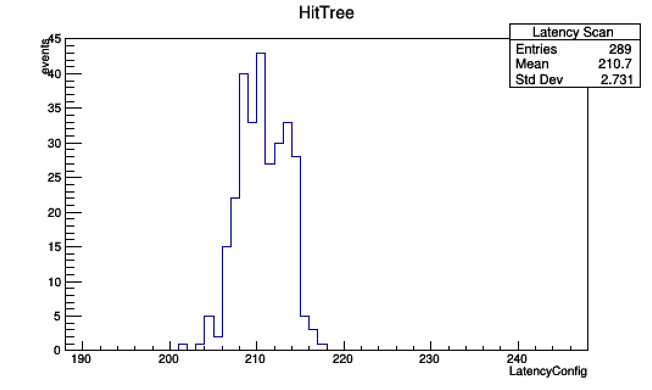
\includegraphics[width=14cm]{./figure/latencydist.png}
  \caption{''LatencyConfig''値とL1ID $== 7$だったイベント数の関係}
  \label{fig:latencydist}
\end{figure}


\subsubsection{Latencyチューニングが幅を持つ理由}
理想的には,Latencyチューニングを行なった時の分布は,正しいLatency値にのみピークが立つはずであるが,今回の結果はそうはなっていない.理由は2つある.
\begin{itemize}
\item YARRの仕組みとして,32bitに1回トリガを発行するかどうかを決めているので,前後8 $\mathrm{Clock}$分の幅が生じる
\item アナログアウトプットのキャパシタンスにズレがあるために前後2 $\mathrm{Clock}$分の幅が生じる.これは,アナログスキャンを行なった時のL1IDの分布を見ると,$\mathrm{L1ID} == 7$のところにのみピークが立つのではなく,前後に2 $\mathrm{Clock}$分の幅を持っていることから確認できる.
\end{itemize}

\section{セルフトリガを用いた応答試験セットアップ}
\label{sec:selfsetup}
主なセットアップは読み出しシステムの動作確認時の図\ref{fig:setup}と変わらず,RD53A搭載のSingle Chip Card(SCC)とFPGAボード,PCを用いて読み出しシステムを構成し,SCCとFPGAボードはアダプタカードを用いてディスプレイポートケーブルによって接続した.センサからの信号を外部に出力するためのコネクタをアダプタカードのport D,RD53Aがコマンドを受け取るためのコネクタをアダプタカードのport Aに繋ぐようにしている.

\section{応答試験手順}
\label{sec:selfhow}
前章で述べたHitOR信号の伝達確認を行なったのち,前節で述べたLatencyチューニングをセンサの上に線源を配置してから行った.''LatencyConfig''の分布が図\ref{fig:latencydist}のように得られたため,今回は''LatencyConfig''の値を211に設定することで,Latencyを合わせた.Latencyを合わせた上で,線源を上をセンサに設置した場合としない場合それぞれについて,30分間のセルフトリガによるデータ取得を行なった.

\section{応答試験結果}
\label{sec:selfconc}
図\ref{fig:self}と表\ref{tab:self}に線源をセンサ上に設置した場合としない場合それぞれの,30分間セルフトリガによるデータ取得結果を示す.

\begin{table}[h]
  \centering
  \caption{線源の有無それぞれのヒットレート}
  \begin{tabular} {|l|c|c||c|} \hline
     & \# Hit & 時間[s] & Hitレート[hits/sec] \\  \hline
    線源なし & $3.528 \times 10^6$ & 1800 & 1960 \\ 
    線源あり & $3.599 \times 10^6$ & 1800 & 2000 \\ \hline
  \end{tabular}
  \label{tab:self}
\end{table}

\begin{figure}[h]
  \centering
  \begin{minipage}[b]{0.45\linewidth}
    \centering
    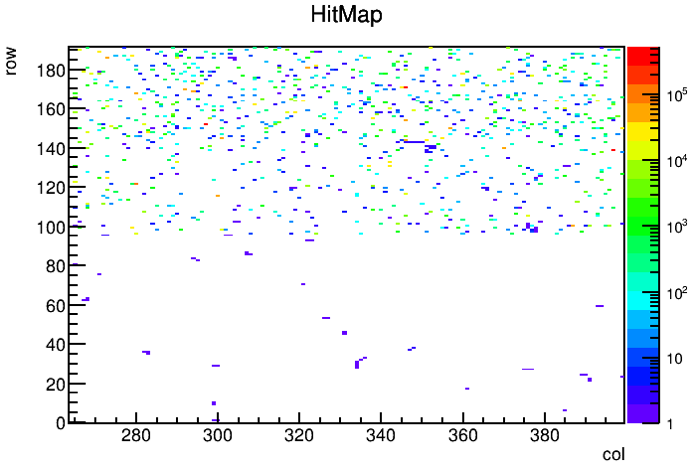
\includegraphics[width=7cm]{./figure/selftrigwo.png}
    \subcaption{線源を置かない場合}
    \label{fig:selfwo}
  \end{minipage}
  \begin{minipage}[b]{0.45\linewidth}
    \centering
    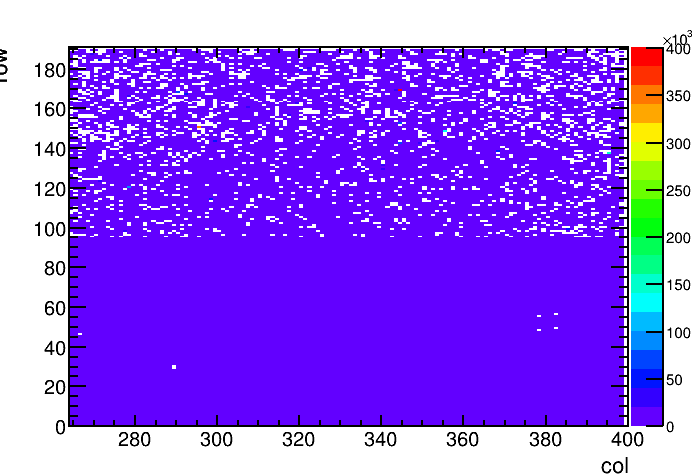
\includegraphics[width=7cm]{./figure/selftrigw.png}
    \subcaption{線源を置いた場合}
    \label{fig:selfo}
  \end{minipage}
  \caption{ヒットの分布}
  \label{fig:self}
\end{figure}

線源あり,なしの場合で,Ocuppancy Mapの分布に差があることが見て取れるが,数値としては,ヒットレートに大きく変化は無かった.応答評価試験として,センサ-ASIC間の接続確認行うためには,センサからの信号でトリガをかけたデータ取得が行われているか確認する必要がある.各ピクセルで線源なし・ありのそれぞれの場合の1ピクセルあたりのHit数分布を図\ref{fig:selfhitfreq}に示す.

\begin{figure}[h]
  \centering
  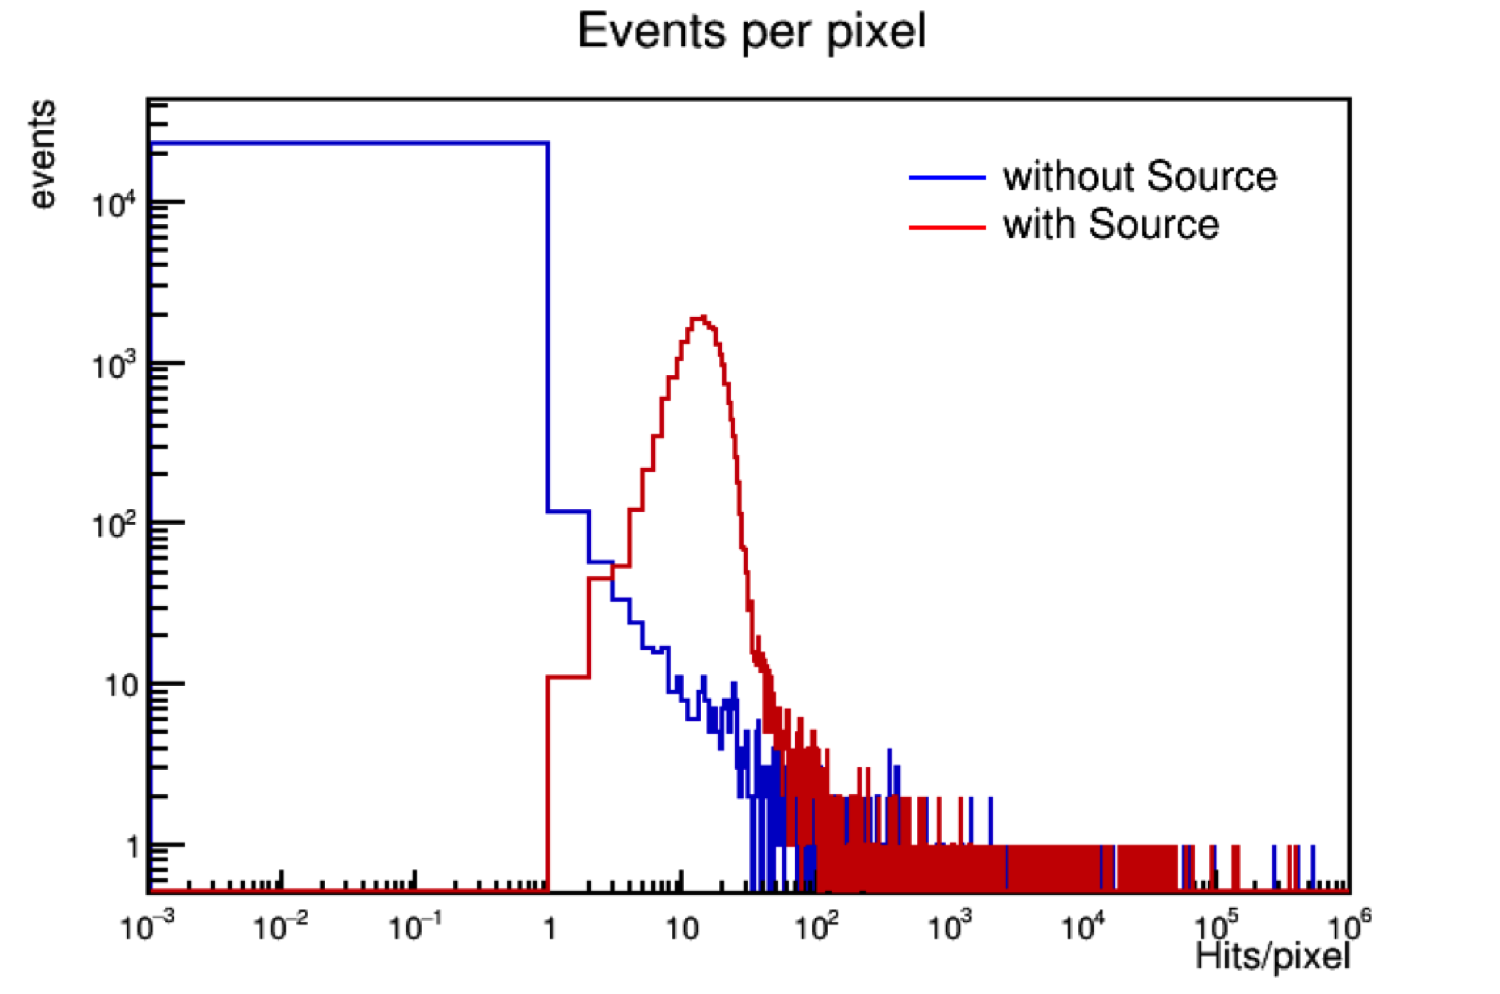
\includegraphics[width=10cm]{./figure/selfhitfreq.png}
  \caption{1ピクセルあたりのHit数分布}
  \label{fig:selfhitfreq}
\end{figure}

このように,線源なしの場合と比較して優位な分布が線源ありの場合に見られる.より詳しく確認するために,以下,線源なしの場合のHit数が0だった場合と,0より大きかった場合に分けて,結果の考察を行なった.

\section{考察}
\label{sec:selfsum}
\subsection*{線源なしの時のHit数が0だった場合}
線源を点線源とみなし,そこから等方的に$\beta$線が放射されていると仮定した場合,今回のセットアップで放射された$\beta$線のうちASICに入射するものの割合を式\ref{eq:beta}を用いて求めた.
\begin{figure}[h]
  \centering
  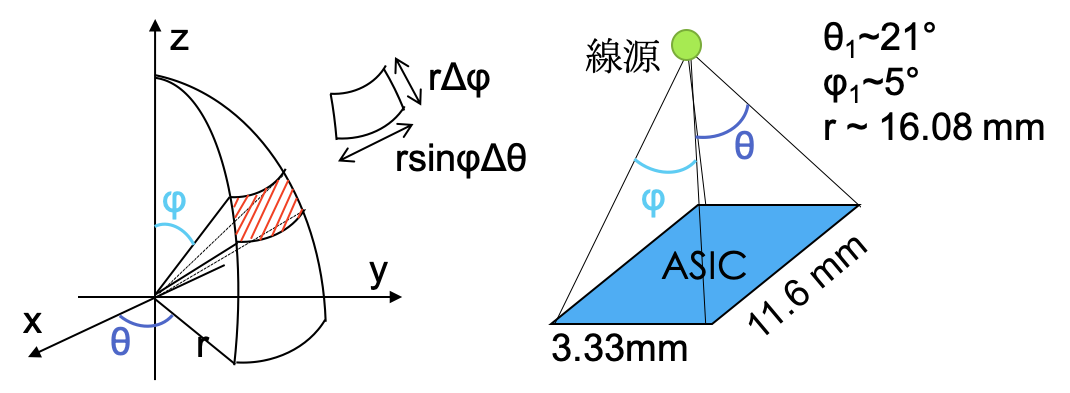
\includegraphics[width=12cm]{./figure/selfarg.png}
  \caption{点線源からの立体角}
\end{figure}

\begin{eqnarray}
  \label{eq:beta}
  \frac{\int^{\phi_1}_0 \int^{\phi_2}_0 r^2 \sin \phi d\theta d\phi}{4 \pi r^2} \simeq 0.28
\end{eqnarray}

本研究で使用したDiff FEのピクセル数が26112,線源の放射能が$4.8 \mathrm{kBq}$であったことから,30分間で1ピクセルが取得できるであろうヒット数を式\ref{eq:hit}のように見積もった.
\begin{eqnarray}
  \label{eq:hit}
  \frac{4.8 \mathrm{kBq} \times 0.28}{26112 \mathrm{pixels}} \times 1800 \mathrm{sec} = 9.18 \mathrm{Hits}
\end{eqnarray}

今回線源からのヒットのデータを取得できていると判断するピクセルの条件を,3ヒットより多くヒットがあったものとした.3ヒットとは,式\ref{eq:hit}より2 $\sigma$の範囲である,$9.18 \times 2 \sqrt{9.18} \simeq 3$から得た値である.線源を置いてデータ取得した場合の1ピクセルあたりのヒット数分布である図\ref{fig:numhitdist}からも,この条件が妥当であることがわかる.この条件を満たし,線源からのヒットがあったと判断したピクセル数を表\ref{tab:0hitdist}に示す.

\begin{figure}[h]
  \centering
  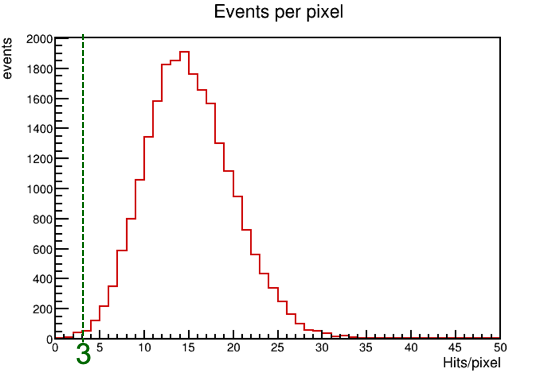
\includegraphics[width=8cm]{./figure/selfperpix.png}
  \caption{線源を置いてデータ取得をした場合の1ピクセルあたりのヒット数}
  \label{fig:numhitdist}
\end{figure}


\begin{table}[h]
  \centering
  \caption{線源からのHitが存在するピクセル数(線源を置いていない時にHit数が0だったピクセルについて)}
  \begin{tabular}{|cl|cl|} \hline
    (i) & 条件を満たすピクセル数 & 22854 & (87.5 \%) \\ \hline
    (ii) & 条件を満たさないピクセル & 56 & (0.2 \%) \\ \hline
  \end{tabular}
  \label{tab:0hitdist}
\end{table}

表\ref{tab:0hitdist}より,30分間のセルフトリガによるデータ取得では,22854個のピクセルが線源からの信号を検出できていると判断できるため,品質保証が可能であることがわかった.一方で,判断できなかった56個のピクセルについては統計量の少なさが原因と考えられるため,今回使用した線源よりも10倍以上強い放射能の線源を用いることで,品質保証が可能になるのではないかと考えた.

\subsection*{線源なしの時のHit数が0より大きかった場合}
線源有り・無しの場合で取得したデータのToT分布を図\ref{fig:selftot}に示す.この分布から,線源からの信号はToT $> 5$に存在すると仮定し,以降ToT $>5$となるデータだけを使用した.バックグラウンドの多いピクセルは,線源からの信号を以下のように見積もり,バックグラウンドの分布と比較した.

\begin{figure}[h]
  \centering
  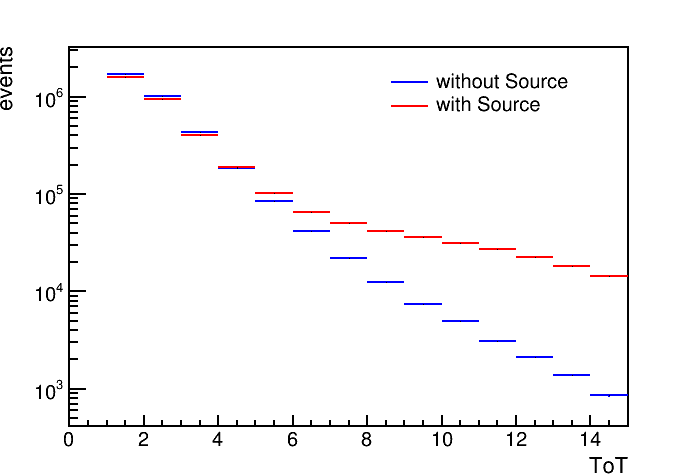
\includegraphics[width=8cm]{./figure/selftot.png}
  \caption{線源の有り(赤)・無し(青)のToT分布}
  \label{fig:selftot}
\end{figure}


\begin{table}[h]
  \centering
  \caption{線源からの信号の分布の見積もり}
  \label{tb:selfnon0}
  \begin{tabular}{cc} \hline
    $n \pm \sqrt{n}$ & 実測値  (線源ありの時のToT $>5$だったピクセルのヒット数) \\
    $n_{bg} \pm \sqrt{n_{bg}}$ & バックグラウンド  (線源なしの時のToT $>5$だったピクセルのヒット数)\\
    $n_{sig} = n - n_{bg}$ & 見積もった真の線源からのヒット数 \\ \hline
  \end{tabular}
\end{table}

表\ref{tb:selfnon0}のように,真の線源からのヒット数を見積もった上で,線源からのヒットがあったとみなすピクセルの条件を式\ref{eq:non0}のように定義した.この条件を満たし,線源からのHitがあったと判断したピクセルの分布を表\ref{tab:non0dist}に示す.

\begin{eqnarray}
  \label{eq:non0}
  \frac{n_{sig}}{\sqrt{n_{bg}}} > 5
\end{eqnarray}

\begin{table}[h]
  \centering
  \caption{線源からのHitが存在するピクセル数(線源を置いていない時にHitが存在したピクセルについて)}
  \begin{tabular}{|cl|cl|} \hline
    (i) & 条件を満たすピクセル数 & 880 & (3.4 \%) \\ \hline
    (ii) & 条件を満たさないピクセル & 77 & (0.3 \%) \\ \hline
  \end{tabular}
  \label{tab:non0dist}
\end{table}

表\ref{tab:non0dist}より,30分間のセルフトリガによるデータ取得では,880個のピクセルが線源からの信号を検出できていると判断できるため,品質保証が可能であることがわかった.一方で,判断できなかった77個のピクセルはバックグラウンドに対して優位な信号を測定することができなかった.センサからの信号でトリガをかけるセルフトリガによるデータ取得方法ではなく,外部トリガによるデータ取得の方でなら,品質保証ができるのではないかと考えた.

\subsection*{まとめ}
30分間のセルフトリガによるデータ取得によって,線源からの信号が取得できたと判断でき,品質保証が可能だったピクセルの分布を表\ref{tab:selfconc}に示す.

\begin{table}[h]
  \centering
  \caption{30分間のセルフトリガによるデータ取得の結果分布}
  \label{tab:selfconc}
  \begin{tabular}{cc} \hline
    90.9 \% & 線源からの信号が検出できた \\
    0.2 \% & 統計量が少なく判断できない \\
    0.3 \% & バックグラウンドに対して有意な信号が検出できない \\
    8.6 \% & ノイズスキャンの段階で非使用と判断されたため判断できない \\ \hline
  \end{tabular}
\end{table}

    


\chapter{外部トリガを用いた応答評価試験}
この章では,外部トリガを用いた粒子線に対する応答評価試験について述べる.\ref{sec:extsetup}節で外部トリガでデータ取得をする際のセットアップ,\ref{sec:exthow}節で手順,\ref{sec:extconc}節で取得データ結果を示し,\ref{sec:selfsum}節で考察を行なっている.

\section{外部トリガを用いた応答評価試験概要}
この節では,4chip-RD53Aモジュールに対して行われる品質試験について述べる.\ref{sec:masspro}節で述べたように,現在現在実機で用いるモジュールを量産するための準備として,プロトタイプ版のASICが4 $\mathrm{Chip}$搭載された4chip-RD53Aモジュールで量産体制の確認が計画されている.この時に,バンプボンディングに異常が無いかを確認するための試験が,外部トリガを用いた応答評価試験である.現在計画されている試験は,クーリングボックスと呼ばれる,温度が低温に維持された小さな箱の中で行い,トリガには前章で述べたHitOR信号ではなく,シンチレータからの光信号を用いる.計画されている外部トリガを用いた応答評価試験セットアップを図\ref{fig:trigplan}に示す.

\begin{figure}[h]
  \centering
  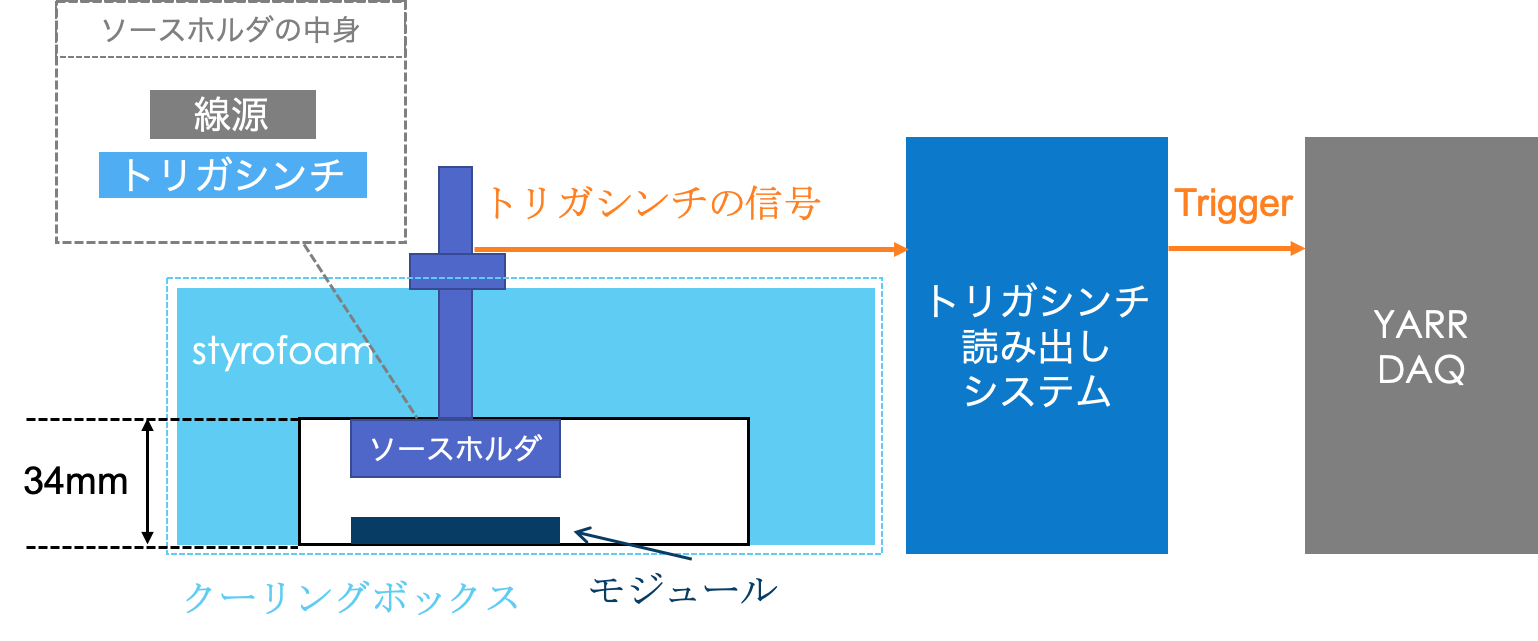
\includegraphics[width=12cm]{./figure/trigplan.png}
  \caption{計画されている外部トリガを用いた応答評価試験セットアップ}
  \label{fig:trigplan}
\end{figure}


線源とモジュールの間にシンチレータを配置し,そのシンチレータに粒子が入射した時の発光をMPPCで検出し信号として読み出すことで,トリガに用いる.このシンチレータとMPPCが合わさったものを以降トリガシンチと呼ぶ.トリガシンチは非常にコンパクトな環境で用いられることや,線源とモジュールの間に配置されることから,なるべく小さく,粒子線を遮ることのないように薄くあることが要求されている.このセットアップで可能な外部トリガを用いた応答評価試験の手法を考える.

\subsection*{MPPC}
MPPCとは,Silicon Photomultipliers(SiPM)と呼ばれるデバイスの一種であり,複数の半導体光検出器・アバランシェフォトダイオード(APD)から成るフォトンカウンティングデバイスである.本論文で用いたMPPC・HAMAMATSU S13360-1325CSは,$1.3 \times 1.3 \mathrm{mm^2}$の受光面に$25 \times 25 \mathrm{\mu m^2}$のAPDが敷き詰められている.MPPCの構成を図\ref{fig:APD}に示す.

\begin{figure}[h]
  \centering
  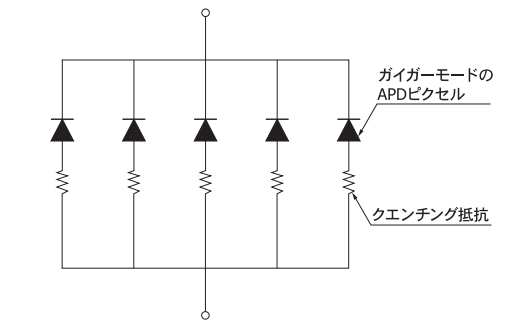
\includegraphics[width=8cm]{./figure/apd.png}
  \caption{MPPCの構成}
  \label{fig:APD}
\end{figure}

全てのAPDの読み出し線,および電圧供給の線は共通していて,全てのAPDピクセルからのシグナルの総和が1つのMPPCからの出力として得られる構造になる.MPPCでは各APDピクセルからの応答が良く揃っているために、総和として出力されるシグナル$Q_{total}$は式\ref{eq:photon}で示されるように光子を受光したピクセル数$N$に1つのAPDから得られるシグナル$Q$をかけた値となる

\begin{eqnarray}
  Q_{total} = N \times Q
\end{eqnarray}

受光したピクセル数は、光が微弱である時入射する光量に比例するため, MPPCは非常に高いフォトンカウンティング能力を備えている.

\subsection*{シンチレータ}
シンチレータとは,放射線のエネルギーを吸収し,内部で励起あるいは電離が起こることで発光する物質である.材質には,無機結晶や液体など様々あるが,本論文では,プラスチックシンチレータを用いた.

\section{トリガシンチの基礎測定}
この節では,RD53Aに対して行われる品質試験で外部トリガとして使用されるトリガシンチの性能の基礎測定について述べる.

\subsection{概要}
今回使用したシンチレータと,光を読み出すためにMPPCをシンチレータに取り付けた様子を図\ref{fig:scin}に示す.図中のライトガイドとは,シンチレータに粒子が入射した時に発光した光を効率よくMPPCまで伝えるための部品である.また,\ref{sec:trigplan}でも述べたように,非常にコンパクトな環境での利用を目的としているため,トリガシンチは箱の中,読み出し回路は箱の外で使用される.そのため,MPPCの足は約30 $\mathrm{cm}$のケーブルをはんだづけすることで延長し,MPPCからの信号を箱の外まで伝えられるようにしてある.シンチレータは0.5 $\mathrm{mm}$と非常に薄いものを使用し,MPPCと共に黒テープで遮光を行なった.

\begin{figure}[h]
  \centering
  \begin{minipage}[b]{0.45\linewidth}
    \centering
    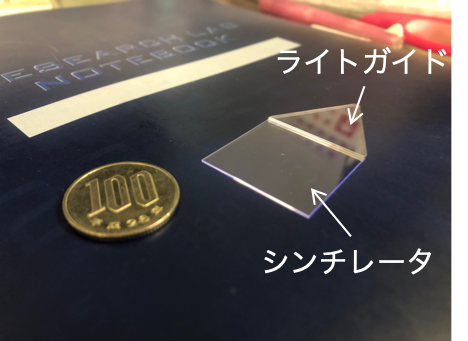
\includegraphics[width=6cm]{./figure/trigscin.png}
    \subcaption{使用したシンチレータとライトガイド}
    \label{fig:scin}
  \end{minipage}
  \begin{minipage}[b]{0.45\linewidth}
    \centering
    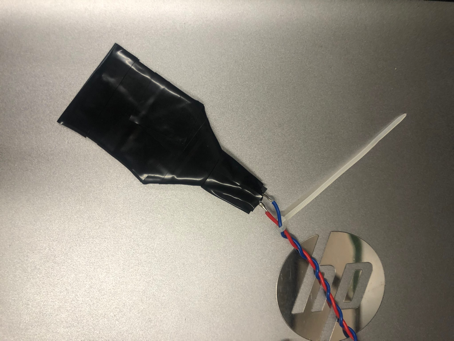
\includegraphics[width=6cm]{./figure/trigscin1.png}
    \subcaption{MPPCを取り付け,遮光したトリガシンチ}
    \label{fig:trigscin}
  \end{minipage}
  \caption{0.5mmのシンチレータの様子}
  \label{fig:trigscin1}
\end{figure}


このトリガシンチに対して以下の2点に関する基礎測定を行なった.
\begin{itemize}
\item 線源を置いた時と置かない時のトリガレート 
\item MPPCが読み出した光量と粒子線が入射した位置の依存性
\end{itemize}

また,今回は使用が予定されている環境がコンパクトな環境なため,ライトガイドを用いた場合と用いなかった場合で,トリガレートや光量に差がないのであれば,ライトガイドはない方が望ましい.よって,ライトガイドが無い場合についても同様の点について基礎測定を行なった.

\subsection{基礎測定のセットアップ}
図\ref{fig:trigsetup}に読み出しシステムの概要を示す.主に,シンチレータとMPPC,読み出し基板,ADCモジュールで構成している.シンチレータで発光した光をMPPCで検出し,読み出し回路でデジタル信号として読み出す.読み出し基板とADCモジュールはコネクタを通してLEMOケーブルで接続している.

\begin{figure}[h]
  \centering
  \includegraphics[width=15cm]{./figure/trigsetup.png}
  \caption{トリガシンチの基礎測定セットアップ}
  \label{fig:trigsetup}
\end{figure}

\subsubsection*{トリガシンチの信号を波形整形する基板}
本研究を行うにあたって,MPPCからの信号を波形整形する基板を作成した.基板を図\ref{fig:extcircle}に示す.主に,電圧供給回路,反転増幅回路,コンパレータ回路,LVDS変換回路から構成されている.基板はKiCADというCERN開発のオープンソースプリント基板CADを用いて設計・作成した.LEMO1からは増幅されたMPPCのアナログ信号を,LEMO2からはコンパレータによって閾値電圧と比較することで変換されたデジタル信号を,DPからはTTLだったデジタル信号が変換されてLVDS出力のデジタル信号を読み出すことができる.その3点についてオシロスコープで観測した波形を図\ref{fig:extosiro}に示す.基礎測定では,LEMO2の出力からGATE信号を生成し,LEMO1の出力のデータを測定した.

\begin{figure}[h]
  \centering
  \begin{minipage}[b]{0.45\linewidth}
    \centering
    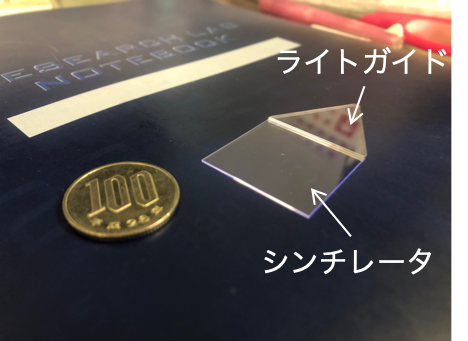
\includegraphics[width=6cm]{./figure/trigscin.png}
    \subcaption{基板の様子}
    \label{fig:pcb}
  \end{minipage}
  \begin{minipage}[b]{0.45\linewidth}
    \centering
    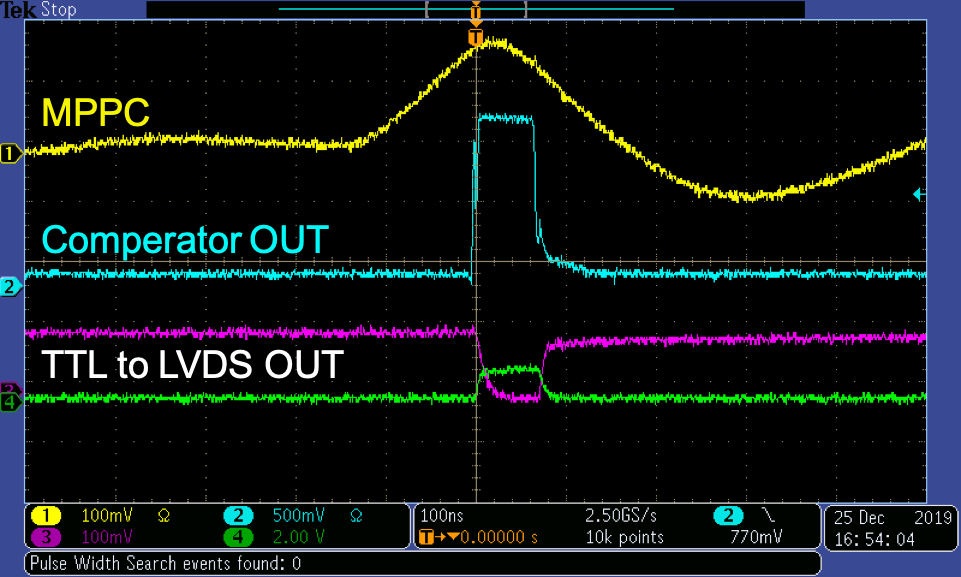
\includegraphics[width=8cm]{./figure/pcbosiro.png}
    \subcaption{動作確認したオシロスコープの様子}
    \label{fig:extosiro}
  \end{minipage}
  \caption{トリガシンチの信号を波形整形する基板}
\end{figure}

\subsection{光量と粒子の入射位置の依存性測定}
粒子の入射位置がMPPCから最も離れている時と,最も近い時で,トリガシンチの読み出す光量にどれくらいの差が出るのかをライトガイドがある場合とない場合で測定した.ライトガイドの必要性を評価するためにこの測定を行なった.

\subsubsection*{手順}
測定を行なった時のトリガシンチと粒子の入射位置を図\ref{fig:trigscinlg}に示す.粒子の入射位置は,トリガシンチと線源の間に小さな穴の空いた鉄板を設置することで調節した.鉄板の穴の位置がMPPCから最も離れている時(図中A)と,最も近い時(図中B)で,トリガシンチから読み出された光量を測定した.ライトガイドありの場合となしの場合で,位置による光量の差に変化があるかを測定した.コンパレータの比較電圧$V_{ref}$を150 $\mathrm{mV}$に設定した.

\begin{figure}[h]
  \centering
  \begin{minipage}[b]{0.45\linewidth}
    \centering
    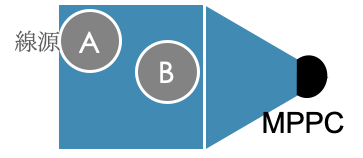
\includegraphics[height=2cm]{./figure/trigscinwlg.png}
    \subcaption{ライトガイドがある場合}
    \label{fig:trigscinwlg}
  \end{minipage}
  \begin{minipage}[b]{0.45\linewidth}
    \centering
    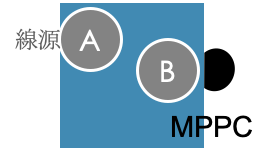
\includegraphics[height=2cm]{./figure/trigscinwolg.png}
    \subcaption{ライトガイドがない場合}
    \label{fig:trigscinwolg}
  \end{minipage}
  \caption{トリガシンチと粒子の入射位置の関係}
  \label{fig:trigscinlg}
\end{figure}

\subsubsection*{結果}
測定結果は図\ref{fig:trigscincon}のようになっている.

\begin{figure}[h]
  \centering
  \begin{minipage}[b]{0.45\linewidth}
    \centering
    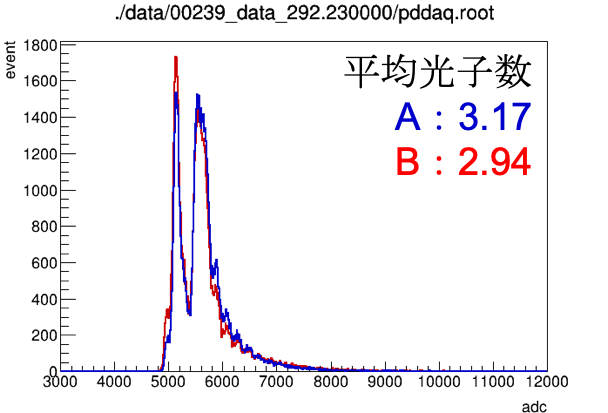
\includegraphics[width=7.5cm]{./figure/trigscinwlgcon.png}
    \subcaption{ライトガイドがある場合}
    \label{fig:trigscinwlg}
  \end{minipage}
  \begin{minipage}[b]{0.45\linewidth}
    \centering
    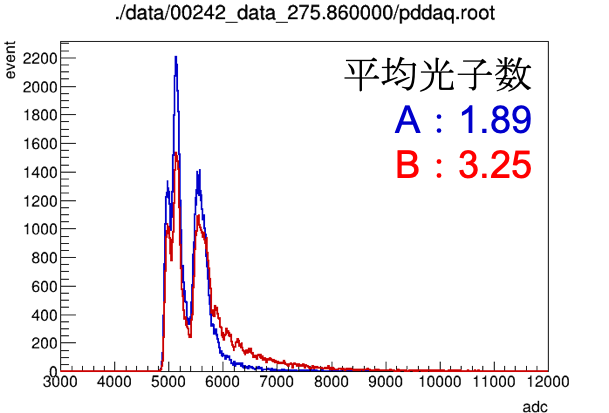
\includegraphics[width=7.5cm]{./figure/trigscinwolgcon.png}
    \subcaption{ライトガイドがない場合}
    \label{fig:trigscinwolg}
  \end{minipage}
  \caption{トリガシンチと粒子の入射位置の関係}
  \label{fig:trigscinlgcon}
\end{figure}



\subsection{トリガレートの測定}
トリガシンチの上に線源を配置した時としない時で,どれくらい
\subsubsection*{手順}
トリガシンチの上に線源を配置した時としない時で,100000イベントのデータを取得するのにかかる時間を測定した.

\subsubsection*{結果}
トリガシンチの上に線源を配置した時としない時のトリガレートの比較結果は表\ref{tab:trigscinrate}のようになっている.

\



\section{外部トリガを用いた応答評価試験セットアップ}
\label{sec:extsetup}
RD53Aの量産にあたって,行われる品質試験では,外部トリガを用いた応答評価試験が行われる.そのため,実際に行われる試験環境に近いセットアップで試験を行なった.セットアップの写真を以下に示す.MPPCには58$\mathrm{V}$印加した.SCCとFPGAボード,PCを用いてシステムを組む大枠は変わらずに,線源の配置とトリガに使用するものが異なっている.\par
実際に行われる試験は,クーリングボックスと呼ばれる,温度が低温に維持された小さな箱の中で行い,トリガには前章で述べたHitOR信号ではなく,シンチレータからの光信号を用いる.シンチレータは線源とモジュールの間に設置するため,なるべく$\beta$線を遮らないように,厚みは0.5$\mathrm{mm}$と非常に薄いものを使用した.
実際に行われる試験環境はクーリングボックスと呼ばれる,温度が低温に維持された小さな箱の中で行う.それに合う応答評価試験セットアップを考えるにあたって,線源とシンチレータ,シンチレータの光信号を電気信号に変換するMPPCが乗ったソースホルダと,MPPCからのアナログ信号を波形整形し,LVDSのデジタル信号に変換するような基板の設計を行なった.

\subsection{ソースホルダの設計}
ソースホルダの外観を以下に示す.クーリングボックス内で使用することを想定し,コンパクトな作りになっている.これは,FreeCADというオープンソース汎用3D CADモデラで設計し,3Dプリンタを用いて作成した.

\subsection{MPPCからの信号を波形整形する回路}

\subsubsection*{回路の動作確認}
MPPCからの信号を正しく波形整形できているかをオシロスコープを用いて確認した.増幅されたMPPCからの信号がコンパレータによって,デジタル信号に変換され,TTL to LVDS変換のチップによって,差動信号に変換されている様子がわかる.

\section{トリガシンチの基礎測定}
この回路では,信号を出力をコンパレータの閾値によって設定している.この閾値によって,MPPCからの信号が削られることなく伝達されているかを確認した.

\section{応答評価試験手順}
\label{sec:exthow}
\section{応答評価試験結果}
\label{sec:extconc}
\section{考察}
\label{sec:extsum}

\chapter{Conclusion}


\chapter*{謝辞}

本研究を進める上でお世話になった方々にお礼申し上げます.指導教員である河野能知准教授には,研究の機会と環境を与えていただきました.また,素粒子実験に関わる知識だけでなくファームウェア,ソフトウェア,回路設計などのノウハウや,研究発表にあたって見やすく伝わりやすい資料作りについてご指導いただきました.毎週の研究室のミーティングでは,研究方針および手法について的確な指摘をいただき,研究をすすめることができました.心から感謝申し上げます.また,副指導教員で本論文の副査を務めていただきました高橋遼助教授にも感謝申し上げます.\par
ATLAS日本QA/QCグループの皆様に感謝いたします.大阪大学の廣瀬穣さんには,ミーティングの場だけでなく,ミーティング外でも時間をとって,ファームウェアの知識のない私に丁寧にご指導いただきましたことに感謝申し上げます.また,東京工業大学の生出秀行さんにも,ソフトウェアの開発やソースホルダの作成の際にたくさんのアドバイスをいただきました.感謝いたします.また,東工大の窪田ありささん,阪大の山家谷昌平さんには,同期として研究姿勢について多くを学ばせていただきました.東工大の松崎貴由さん.池亀遥南さんには,クーリングボックスにソースホルダを組み込むにあたって設計についての相談にのっていただきました.東工大の奥山広貴さんにはデータベースの使い方を丁寧に教えていただき,また阪大のLakmin Wickremasingheさんには回路設計についてアドバイスをいただきました.\par
お茶の水女子大学河野研究室の皆様に感謝申し上げます.藤本みのりさんには,データ取得を手伝っていただいたこと,ファームウェアとソフトウェアについての多くの知識を教えていただきました.浅井香奈江さんには,コーディング技術や,プロットの見せ方について多くの助言をいただきました.河野研究室卒業生の里吉陽奈子さんには,見やすい発表資料の作り方について大変参考にさせていただきました.また修士1年で同じATLAS日本QA/QCグループだった,釣希夢さん,前田実津季さんには発表資料や実験方針,ソフトウェアの設計など,多くの相談にのっていただき,大変感謝しています.\par
ATLASグループでは,KEKの中村浩二さん,筑波大学の原田大豪さんには,センサについての知識を教えていただいた上に,データ取得するにあたって多くの時間をとって協力してくださり大変感謝しています.また,東工大の金恩寵さん,潮田理沙さん,卒業生の中村優斗さんには学会などで会うたびによくしてくだいました.ありがとうございました.\par
最後に,何不自由ない学生生活,研究生活を実現してくたださった両親に深く感謝いたします.




\bibliography{./bib/IOPEXPORT_BIB}
\bibliographystyle{junsrt}
%\bibliography{./bib/HLLHC_BIB}
%\bibliography{./bib/ITK_BIB}

\appendix

\listoffigures
\listoftables

\end{document}

